
\section{Introduction to Neural Networks}
\newcommand{\derl}{\mathrm{\delta^\ell}}
\newcommand{\derL}{\mathrm{\delta^L}}
\newcommand{\derlj}{\mathrm{\delta^\ell_j}} 
\newcommand{\derLj}{\mathrm{\delta^L_j}} 
\newcommand{\derLn}{\mathrm{\delta^{L+1}}}
\newcommand{\derln}{\mathrm{\delta^{l+1}}}
\newcommand{\derLkn}{\mathrm{\delta_k^{L+1}}} 
\newcommand{\derlkn}{\mathrm{\delta_k^{l+1}}} 
\newcommand{\derCL}{\mathrm{\frac{\partial C}{\partial a_j^L}}}
\newcommand{\derCl}{\mathrm{\frac{\partial C}{\partial a_j^\ell}}}

Artificial neural networks have been around for a long time, since 1943 when in the paper, "A Logical Calculus of Ideas Immanent in Nervous Activity" McCulloch and Pitts presented a simplified computational model of how biological neurons might work together in animal brains to perform complex computations using propositional logic. The early successes of ANNs until the 1960s led to the widespread belief that we would soon be conversing with truly intelligent machines but the promise went unfulfilled. During the early 1980s there was some slow progress but in the 1990s more promising algorithms arrived, especially SVM. Only recently they have finally caught on due to the high volume of data available, increase of computing powers and especially GPU, better training algorithms and because some theoretical limitations, such as getting stuck in local minima, have turned out to rarely happen in practice.

The mechanism of a biological neuron is very simple, but the network it belongs to is very complex. McCulloch and Walter Pitts proposed a very simple model of the biological neuron, which later became known as an artificial neuron: it has one or more binary (on/off) inputs and one binary output. The artificial neuron simply activates its output when more than a certain number of its inputs are active. McCulloch and Pitts showed that even with such a simplified model it is possible to build a network of artificial neurons that computes any logical proposition you want.

\footnote{\url{http://neuralnetworksanddeeplearning.com/chap1.html}} One of the first artificial neuron is the \tb{perceptron}, which was modelled in the 1950s and 1960s by Frank Rosenblatt, inspired by Warren McCulloch and Walter Pitts. A perceptron takes several real-valued inputs, $x_1, x_2,\cdots$ and produces a single binary output. Rosenblatt introduced \tb{weights} $w_1, w_2, \cdots$, real number expressing the importance of each input in relation to the output. The neuron's output can be only $0$ or $1$ and it is determined whether the weighted sum of the inputs is less or greater than a threshold value:
\begin{equation}
output \systeme*{0 \textit{ if } {\sum_j w_j x_j \le \ti{threshold}} ,1 \textit{ if } {\sum_j w_j x_j> \ti{threshold}}}
\end{equation}
which is equivalent to 
\begin{equation}
output \systeme*{0 \textit{ if } {\sum_j w_j x_j+b \le 0} ,1 \ti{ if } {\sum_j w_j x_j +b> 0}}
\label{eq:PerceptronInequalities}
\end{equation}
where $b$ is termed the bias. One can think of the bias as a measure of how easy it is to get the perceptron to output a $1$. Or to put it in more biological terms, the bias is a measure of how easy it is to get the perceptron to fire. For a perceptron with a really big bias, it's extremely easy for the perceptron to output a $1$. But if the bias is very negative, then it's difficult for the perceptron to output a $1$.
Also we can express the weighted sum as a dot product: $\sum_j w_j x_j \equiv w \cdot x$
A way you can think about the perceptron is that it's a device that makes decisions by weighing up evidence. By varying the weights and the threshold, we can get different models of decision-making. 

Although simple, this model can be extended to a more complex network able to make subtle decisions. In such a network, the first layer (apart the input layer which although sometimes is depicted as with neurons, it is not actually so) of perceptrons weights the inputs as if they were making multiple decisions and these results are used as inputs of the second layer to make more abstract decisions and so on.

Despite decision making, another way perceptrons can be used is to compute the elementary logical functions, such as AND, OR, and NAND. For example, suppose we have a perceptron with two inputs, each with weight $-2$, and an overall bias of $3$. It can be easily proved that this represents a NAND gate. Furthermore, we can use networks of perceptrons to compute any logical function at all. The reason is that the NAND gate is universal for computation, that is, we can build any computation up out of NAND gates.

Perceptrons can also be thought of as a simple linear binary classifier. If the result exceeds a threshold, it outputs the positive class or else outputs the negative class. 

The view of perceptrons as a computing device although interesting it does not add anything more to the already existing NAND gates. However, it turns out that we can devise learning algorithms which can automatically tune the weights and biases of a network of artificial neurons. This tuning happens in response to external stimuli, without direct intervention by a programmer. These learning algorithms enable us to use artificial neurons in a way which is radically different to conventional logic gates.

\subsection{Clarification about local optima in high dimensional space}
In a Neural Network, most of the points with gradient equal to $0$ are not local optima but saddle points \autoref{img:saddle}. Saying that a function has zero gradient means that in each direction it can either be a convex or concave function. If the function is a very high dimensional space, then for it to be a local optima, all the directions need to be convex. The chance of that happening is very very small and one is much more likely to et some directions where the curve forms a saddle point. To explain this, suppose a function has 2000 dimensions and in one point the gradient is $0$. Assuming that in a single dimension it can be convex or concave with the same probability of $0.5$, then the probability of the point being a local optimum is $2^{-2000}$. Althogh informal, this reasoning can give some intuitions why local optima in high dimensional space are much rarer tha expected.

\begin{figure}
\centering
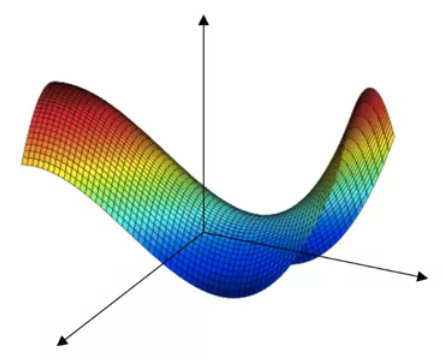
\includegraphics[scale=0.6]{img/saddle}
\caption{Example of a saddle point where the derivatives are all zeros.}
\label{img:saddle}
\end{figure}


Rather than local optima, plateaus are responsible for slowing the training. Plateaus are regions where the derivatives are close to $0$ for a long time \autoref{img:plateau}. Algorithms like Momentum (\autoref{subsec:momentum}), RMSProp (\autoref{subsec:RMSprop}) or ADAM (\autoref{subsec:ADAM} can really help learning algorithm in these cases.

\begin{figure}
\centering
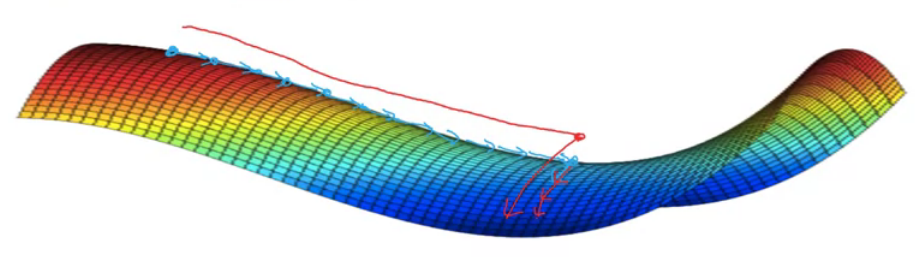
\includegraphics[scale=0.4]{img/plateau}
\caption{Example of a plateau with derivative close to $0$ in all directions. It might happen the algorithm slowly travels all the plateau before following a steeper direction.}
\label{img:plateau}
\end{figure}

To conclude, consider that hardly anyone has great intuitions about what these spaces look really like.

\subsection{Sigmoid neurons and Gradient descent technique}
\subsubsection{Sigmoid neurons}
To see how learning might work, suppose we make a small change in some weight (or bias) in the network. What we'd like is for this small change in weight to cause only a small corresponding change in the output from the network: this property will make learning possible. Schematically, here's what we want
\begin{figure}
\centering
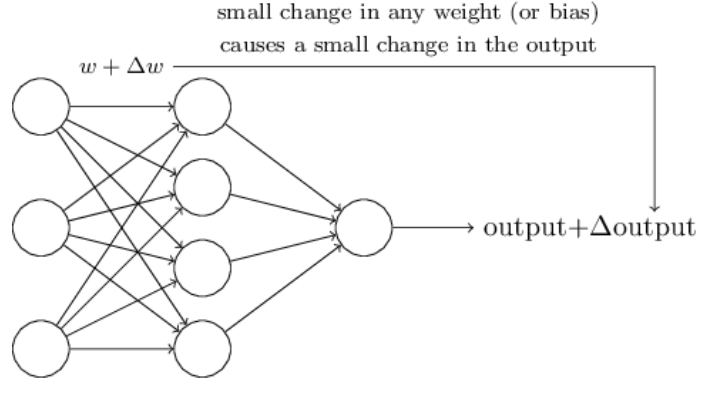
\includegraphics[scale=0.4]{img/NNdeltaChange}
\caption{Desired behaviour to make learning possible for a network of artificial.}
\label{NNdeltaChange}
\end{figure}

Given that, we could use this fact to modify the weights and biases to get our network to behave more in the manner we want. For example, suppose the network was mistakenly classifying an image as an "8" when it should be a "9". We could figure out how to make a small change in the weights and biases so the network gets a little closer to classifying the image as a "9". And then we'd repeat this, changing the weights and biases over and over to produce better and better output. The network would be learning. The problem is that this isn't what happens when our network contains perceptrons. In fact, a small change in the weights or bias of any single perceptron in the network can sometimes cause the output of that perceptron to completely flip, say from $0$ to $1$. That flip may then cause the behaviour of the rest of the network to completely change in some very complicated way. So while your "9" might now be classified correctly, the behaviour of the network on all the other images is likely to have completely changed in some hard-to-control way. That makes it difficult to see how to gradually modify the weights and biases so that the network gets closer to the desired behaviour.

We can overcome this problem by introducing a new type of artificial neuron called a \tb{sigmoid neuron}. Sigmoid neurons are similar to perceptrons, but modified so that small changes in their weights and bias cause only a small change in their output. That's the crucial fact which will allow a network of sigmoid neurons to learn. In such an artificial neuron, instead of being just $0$ and $1$, the output can take any other value in the range $[0,1]$. As its predecessor, it still has weights and biases. Its output though is calculated as:
\begin{equation}
\begin{aligned}
\textit{output} = \sigma(w\cdot x+b) = \sigma(z) = \frac{1}{1+e^{-z}} = \frac{1}{1+e^{-\sum_j x_j \cdot w_j -b}} 
\end{aligned}
\end{equation}
As already presented in \autoref{LogReg}, the sigmoid gets close to $1$ for large inputs and close to $0$ for small ones (close to $-\infty$). Said in other words, its behaviour is not so different from the perceptron. The deviation between the two functions is when $w\cdot x +b$ has modest size, where the sigmoid has a smooth behaviour while the perceptron acts as a step function. It's the smoothness that ensures that small changes in the weights and biases give small changes in the output.

In \autoref{subsec:Taylor} it was shown how a multi-variable scalar function can be approximated to a first order polynomial around a given point. Considering a single neuron as a function $f$ of input weights $w_j$, bias $b$, and a scalar output, its approximation around $(w^{(0)}, b^{(0)})$ is (separating the contribution of weights and biases):
\begin{equation}
\begin{aligned}
f(w_j, b) &\approx f(w_j^{(0)}, b^{(0)})+ \sum_ j\frac{\partial f}{\partial w_j} \left(w_j-w_j^{(0)}\right) +\frac{\partial f}{\partial b} \left(b-b^{(0)}\right) \Rightarrow\\
&\Rightarrow f(w, b) - f(w_j^{(0)}, b^{(0)} )= \Delta output \approx \sum_ j\frac{\partial f}{\partial w_j} \Delta w +\frac{\partial f}{\partial b} \Delta b
\end{aligned}
\label{eq:NNsmallChanges}
\end{equation}
This linear relationship makes it easy to choose small changes in the weights and biases to achieve any desired small change in the output. So, while sigmoid neurons have much of the same qualitative behaviour as perceptrons, they make it much easier to figure out how changing the weights and biases will change the output.

Other activation functions exist as well. The main difference when using a different activation function is that the particular values for the partial derivatives change. Nonetheless, sometimes one wants the output to be binary. In practice one can set up a convention to deal with the real valued number ranging from $0$ to $1$ and output by the neuron, for example, by deciding to interpret any output of at least $0.5$ as \cd+True+, and the others as \cd+False+.

Note that in a network of perceptions, multiplying all the weights and biases by a positive constant $c$ does not change its behaviour. In fact, each perceptron outputs either $0$ or $1$ according to the inequalities in \autoref{eq:PerceptronInequalities}. Multiplying the weights and biases by a positive constant does not change the inequalities and hence the output of each perceptron does not change.

On the contrary, multiplying all the weights and biases of a network of sigmoid neurons by a positive constant, changes the behaviour of the network. Particularly, if for a neuron $w\cdot x +b \ne 0$, multiplying its weights and bias by a positive constant $c$ and then letting $c\rightarrow \infty$, the behaviour gets closer to the one of a perceptron. There are at least two ways to show this. Consider the mathematical representation of a sigmoid function:
\begin{equation*}
\sigma(cw,cb) = \frac{1}{1+e^{(-wx-b)c}}
\end{equation*}
As $c\rightarrow \infty$, even for small values of $w\cdot x +b$, the sigmoid outputs either $0$ or $1$ since such a small value is multiplied by an infinite quantity. Particularly, it outputs $1$ when $w\cdot x+b\ge 0$, $0$ otherwise. 

Secondly consider this: the behaviour of the sigmoid is already close to the one of the perceptron in the extreme regions but different around $w\cdot x +b \approx 0$, so let us see what happens here and use the Taylor first order approximation (here the sigmoid is not so different from a straight line) and let us consider $\sigma(x)$ for simplicity:
\begin{equation}
\sigma(x) = \frac{1}{1+e^{-cx}} = \frac{1}{2} +  \left. \frac{ce^{-cx}}{\left(1+e^{-cx}\right)^2}\right|_0 (x-0) = \frac{1}{2}+ cx
\end{equation}
As $c\rightarrow \infty$, the piece of the sigmoid around $x=0$ gets closer to a vertical line, like the perceptron.

\subsubsection{The architecture of a neural network}
As mentioned earlier, the leftmost layer in this network is called the \tb{input layer}, and the neurons within the layer are called \tb{input neurons}. The rightmost or output layer contains the \tb{output neurons}, or, as in this case, a single output neuron. Middle layers between the input and output layers are called a \tb{hidden layers}, since the neurons in these layers are neither inputs nor outputs. The term "hidden" perhaps sounds a little mysterious, but it really means nothing more than "not an input or an output". 

Somewhat confusingly, and for historical reasons, multiple layer networks are sometimes called multilayer perceptrons or MLPs, despite being made up of sigmoid neurons, not perceptrons. 

When all the neurons in a layer are connected to every neuron in the previous layer (i.e., its input neurons), it is called a \tb{fully connected} layer or a \tb{dense layer}.

The design of the input and output layers in a network is often straightforward. For example, suppose we're trying to determine whether a handwritten image depicts a "9" or not. A natural way to design the network is to encode the intensities of the image pixels into the input neurons. If the image is a $64$ by $64$ greyscale image, then we'd have $4096=64\times64$ input neurons, with the intensities scaled appropriately between $0$ and $1$. The output layer will contain just a single neuron, with output values of less than $0.5$ indicating "input image is not a 9", and values greater than $0.5$ indicating "input image is a 9 ". The difficulty relies in choosing the hidden layers, for which there is no rule but just some heuristics. 

Up to now, we've been discussing neural networks where the output from one layer is used as input to the next layer. Such networks are called \tb{feedforward neural networks}. This means there are no loops in the network - information is always fed forward, never fed back. If we did have loops, we'd end up with situations where the input to the $\sigma$ function depended on the output. 

However, there are other models of artificial neural networks in which feedback loops are possible. These models are called \tb{recurrent neural networks} or \tb{RNN}. The idea in these models is to have neurons which fire for some limited duration of time, before becoming quiescent. That firing can stimulate other neurons, which may fire a little while later, also for a limited duration. That causes still more neurons to fire, and so over time we get a cascade of neurons firing. Loops don't cause problems in such a model, since a neuron's output only affects its input at some later time, not instantaneously.

Considering a simple handwritten digit NN, generally 10 output neurons are used, each representing a single digit. If such a neuron has a value close to $1$ it means the network considers the image to represent that digit. A seemingly natural way of doing that is to use just $4$ output neurons, treating each neuron as taking on a binary value, depending on whether the neuron's output is closer to $0$ or to $1$. Four neurons are more than enough to encode the answer: $2^4=16$. So why didn't this representation catch on? The ultimate justification is empirical: we can try out both network designs, and it turns out that, for this particular problem, the network with $10$ output neurons learns to recognize digits better than the network with $4$ output neurons. But that leaves us wondering why using $10$ output neurons works better. Is there some heuristic that would tell us in advance that we should use the $10$-output encoding instead of the $4$-output encoding?

Heuristically, the reason can be that hidden neurons encode information about some substructures of the image. For example suppose one of them represent the shape of a $0$ in the top right of the picture, one another the top left and so on. If they fire together it means the image is a $0$, so the mapping is between fragments of the image to a full image representing (or non representing) a digit. If we use just $4$ neurons, it means we are using one output neuron (i.e., one bit) for representing a bit value, not directly an image. For example $0001$ and $0011$ and $0111$ have all the LSB set to $1$ but they represent different images, so it is more difficult to establish a relationship between the substructures encoded by the hidden layers with the outputs. However this is just an interpretation.

\subsubsection{Gradient Descent learning}
What we'd like is an algorithm which lets us find weights and biases so that the output from the network approximates $y(x)$ for all training inputs $x$. To quantify how well we're achieving this goal we use the quadratic cost function:
\begin{equation}
C(\w, b) = \frac{1}{2N}\sum_\x \|y(x)-a \|^2
\end{equation}
where $N$ is the total number of training inputs and $a$ is the vector of outputs from the network for the $\x$ input, which depends also from $\w$ and $b$. Using such a measure instead of a measure that counts directly the number of the images correctly classified guarantees a smooth function on which small changes of the weights and biases can produce an observable change in the output. When using the number of correctly classified images, very often small changes to the parameters do not produce any effect and it is difficult if the network is improving or not.

Being this a quadratic function, its minimization is a well-posed problem. One way of attacking the problem is to use calculus to try to find the minimum analytically. We could compute derivatives and then try using them to find places where $C$ is an extremum. With some luck that might work when $C$ is a function of just one or a few variables. But it'll turn into a nightmare when we have many more variables. And for neural networks we'll often want far more variables - the biggest neural networks have cost functions which depend on billions of weights and biases in an extremely complicated way. Using calculus to minimize that just won't work!

Consider a two-variable cost function $C(v_1, v_2)$. As already seen in \autoref{eq:NNsmallChanges}, we can associate small changes in the output to small changes in the inputs with the relationship:
\begin{equation}
\Delta C \approx \frac{\partial C}{\partial v_1} \Delta v_1 +\frac{\partial C}{\partial v_2} \Delta v_2
\label{NN:eq2varGrad}
\end{equation}
Being it a cost function representing the error, we want to minimize it, i.e. make $\Delta C$ negative by choosing proper values of $\Delta v_i$. Setting $\Delta v \equiv \left( \Delta v_1, \Delta v_2, \right)^T$ and $\nabla C \equiv \left( \frac{\partial C}{\partial v_1}, \frac{\partial C}{\partial v_1}\right)^T$. Then we can rewrite \autoref{NN:eq2varGrad} as:
\begin{equation}
\Delta C \approx \nabla C \Delta v
\end{equation}
We want to make $\Delta C$ negative and to do that we can choose a value of $\Delta v$. Suppose we choose
\begin{equation}
\Delta v = -\eta \nabla C
\end{equation}
with $\eta$ a small positive parameter defined as the \tb{learning rate}. Then
\begin{equation}
\Delta C = -\eta \| \nabla C \|^2
\end{equation}
$ \| \nabla C \|^2$ is a positive quantity, so this guarantees $\Delta C \le 0$, i.e., $C$ will always decrease, never increase, if we change $v$ accordingly. So from the expression of $\Delta v$:
\begin{equation}
v \rightarrow v' = v -\eta \Delta C
\end{equation}
It is like we are moving on the surface of $C$ from our current position $v$ by the quantity and direction $\Delta v$. The result of this step is achieving a point with less "altitude". If we keep doing this, over and over, we'll keep decreasing $C$ until - we hope - we reach a global minimum.

To make gradient descent work correctly, we need to choose the learning rate $\eta$ to be small enough so that the approximation is valid. If we don't, we might end up with $\Delta C > 0$, which obviously would not be good! At the same time, we don't want $\eta$ to be too small, since that will make the changes $\Delta v$ tiny, and thus the gradient descent algorithm will work very slowly. In practical implementations, $\eta$ is often varied so that the approximation is valid, but the algorithm isn't too slow. 

Allowing $C$ to be a function of more than $2$ variable does not change the equations and their meaning, the changes just rely on $\Delta v \equiv $ $\left( \Delta v_1, \cdots, \Delta v_m, \right)^T$ and $\nabla C \equiv$ $\left( \frac{\partial C}{\partial v_1}, \cdots, \frac{\partial C}{\partial v_m}\right)^T$.

The rule doesn't always work - several things can go wrong and prevent gradient descent from finding the global minimum of $C$, but often it works extremely well.

There is even a mathematical sense in which the gradient descent is the optimal strategy for searching for a minimum. As already said we have to look for the minimum $\Delta C \approx \nabla C  \cdot \Delta v$. We constrain $\| \Delta v \| = \epsilon$ for small fixed  $\epsilon > 0$. Using the Cauchy-Schwarz inequality presented in \autoref{sec:CauchySchwarz}, we have:
\begin{equation}
\left| \langle \nabla C, \Delta v \rangle \right|^2 \le \langle \nabla C, \nabla C \rangle\cdot \langle \Delta v, \Delta v \rangle 
\end{equation}
with equality holding only when  the vectors are linear dependent, i.e. $\nabla C = \eta \Delta v$. But instead of maximising it, we want to minimise it, so we take the opposite direction: $\nabla C = -\eta \Delta v$, so that we have:
\begin{equation}
\begin{aligned}
\left| \langle  \nabla C, -\eta  \nabla C \rangle \right|^2 = \|\nabla C\|^2 \cdot \epsilon^2 
\Rightarrow \left( -\eta \|\nabla C\|^2\right)^2 =\|\nabla C\|^2 \cdot \epsilon^2 \Rightarrow \\
\Rightarrow \eta^2 \|\nabla C\|^{\cancel{4}^2} = \cancel{\|\nabla C\|^2} \cdot \epsilon^2
\Rightarrow \eta = \frac{\epsilon}{\|\nabla C\|}
\end{aligned}
\end{equation}
since $\left| \langle  \nabla C, -\eta  \nabla C \rangle \right| = \eta $, $\epsilon = \langle \Delta v, \Delta v \rangle $. This gives the best value of $\Delta v$ with the constraint of $\epsilon$ to its magnitude.

One might ask why not to get a better approximation bringing in also the second derivatives? The answer is that is with second order derivatives it becomes too expensive. For example consider one has $100$ variables. Considering just the first derivatives "only" $100$ derivatives have to be computed. Considering the second derivatives and given that $\frac{\partial^2}{\partial x \partial y} =  \frac{\partial^2}{ \partial y\partial x}$, one gets $100$ second derivatives of the same variables plus $99$ cross-derivatives of the first variable, plus $98$ cross-derivatives of the second variables with the others (except the first) and so on which is equal to $101\cdot 100 /2 = 5050$ (\autoref{sec:SumDecreasingNumber}).

Now we want to apply the Gradient Descent to upload the weights and biases:
\begin{equation}
\begin{aligned}
w_k \rightarrow w_k' &= w_k - \eta \frac{\partial C}{\partial w_k}\\
b_\ell \rightarrow b_\ell' &= b_\ell - \eta \frac{\partial C}{\partial b_\ell}
\end{aligned}
\end{equation}
These rules are applied repeatedly to minimise the function. The cost function is a sum of the single errors over all the training inputs: $C = \frac{1}{2n}\sum_x C_x$. So to calculate $\nabla C$ one has to go through over all the samples, and compute the gradient for each training input and then average them: $\nabla C = \sum_x C_x$. When the number of training is very large, this becomes unfeasible. 

An idea is to use an approximation called \tb{stochastic gradient descent} to speed up learning. The idea is to estimate $\nabla C$ by computing $\nabla C_x$ for a small sample of randomly chosen training inputs. In this way we can quickly get a good estimate of the gradient. So instead of all the samples, we take $m$ training inputs, forming a \tb{mini-batch}. Calling the training inputs $X_j$, if $m$ is large enough we expect:
\begin{equation}
\sum_{j=1}^{m} \nabla C_{X_j}\approx \sum_{x}\nabla C_x =\nabla C
\end{equation}
So the update equations become:
\begin{equation}
\begin{aligned}
w_k \rightarrow w_k' &= w_k - \frac{\eta}{m} \sum_j  \frac{\partial C_{X_j}}{\partial w_k}\\
b_\ell \rightarrow b_\ell' &= b_\ell - \frac{\eta}{m} \sum_j  \frac{\partial C_{X_j}}{\partial b_\ell}
\end{aligned}
\end{equation}
Then we pick out another randomly chosen mini-batch and train with those. And so on, until we've exhausted the training inputs, which is said to complete an \tb{epoch} of training. At that point we start over with a new training epoch.

Incidentally, it's worth noting that conventions vary about scaling of the cost function and of mini-batch updates to the weights and biases. We have scaled the overall cost function by a factor $\frac{1}{n}$. People sometimes omit this factor, summing over the costs of individual training examples instead of averaging. This is particularly useful when the total number of training examples isn't known in advance. This can occur if more training data is being generated in real time, for instance. And, in a similar way, the mini-batch update rules sometimes omit the $\frac{1}{m}$ term out the front of the sums. Conceptually this makes little difference, since it's equivalent to rescaling the learning rate. But when doing detailed comparisons of different work it's worth watching out for.

We still have to compute $\nabla C$.

\subsection{Backpropagation}
The backpropagation algorithm was originally introduced in the 1970s, but its importance wasn't fully appreciated until a famous 1986 paper by David Rumelhart, Geoffrey Hinton, and Ronald Williams. That paper describes several neural networks where backpropagation works far faster than earlier approaches to learning, making it possible to use neural nets to solve problems which had previously been insoluble. Today, the backpropagation algorithm is the workhorse of learning in neural networks.

Let us define $w_{jk}^{\ell}$ as weight from the $k$-th neuron in the layer $\ell-1$ to the $j$-th neuron in the layer $\ell$ and $b^\ell_j$ as the bias of the $j$-th neuron in the layer $\ell$. Finally, let us indicate the output layer as $L$. The activation $a_j^\ell$ of the $j$-th neuron in the $\ell$ layer can be written as:
\begin{equation}
a_j^\ell = \sigma \left(\sum_k w_{jk}^\ell a_k^{\ell-1} + b_j^\ell\right)
\end{equation}
where the sum is over all the $K$ neurons in the $\ell-1$ layer. Using the matrix notation we can represent a full layer:
\begin{equation}
a^\ell = \sigma \left( w^\ell a^{\ell-1} +b^\ell\right)
\end{equation}
\subsubsection{Two assumptions about the cost function}
The goal of backpropagation is to compute the partial derivatives. For backpropagation to work we need to make two main assumptions about the form of the cost function. 
The \tb{first assumption} we need is that the cost function can be written as an average $C=\frac{1}{n}\sum_x C_x$ over cost functions Cx for individual training examples, $x$. This is the case for the quadratic cost function.

The \tb{second assumption} we make about the cost is that it can be written as a function of the outputs from the neural network. Again, the quadratic cost function satisfies this requirement.
\subsubsection{The Hadamard product}
Suppose $s$ and $t$ are two vectors of the same dimension. Then we use $s\odot t$ to denote the vector with the same length whose elements are given by the elementwise product of two vectors.
This is called \tb{Hadamard product} or \tb{Schur product}.

The product is equivalent to a matrix multiplication where the last vector is multiplied by a diagonal square matrix of the same length, whose elements are the elements of the first vector:
\begin{equation}
s\odot t = \Sigma(s) t = \begin{pmatrix} s_1 &0 &\cdots & 0 \\0 & s_2 & \cdots &0 \\
\vdots & \vdots &\vdots & \vdots\\
0  & 0 &0 &s_n
\end{pmatrix}t
\end{equation}

\subsubsection{The four fundamental equations}
Backpropagation is about understanding how changing the weights and biases in a network changes the cost function. Ultimately, this means computing the partial derivatives.

Backpropagation will give us a procedure to compute such an error and relate it to the partial derivatives. Defining $z_j^\ell = \sum_k w_{jk}^\ell a_k^{\ell-1} + b_j^\ell$, suppose one changes the value of $z_j^\ell$ by a small quantity $\Delta z_j^\ell$. This will affect the cost function by a quantity equal to $\frac{\partial C}{\partial z_j^\ell}\Delta z_j^\ell$. If the quantity $\frac{\partial C}{\partial z_j^\ell}$ has a large value, then one can largely improve (decrease) the cost-function by choosing $\Delta z_j^\ell$ to have an opposite direction: the neuron has still room for improvement. On the contrary if $\frac{\partial C}{\partial z_j^\ell}$ is close to $0$, any value for $\Delta z_j^\ell$ is not effective: in this case the neuron does not have room for improvement, or said in other words, it is already optimal. We can associate a measure to how far a neuron is from its optimality, i.e., an error, and this error is represented, apart constants, by $\frac{\partial C}{\partial z_j^\ell}$. Let us define $\delta_j^\ell$ the error in the $j$-th neuron of the $\ell$ layer:
\begin{equation}
\delta_j^\ell =\frac{\partial C}{\partial z_j^\ell}
\end{equation}
One might wonder why changing the weighted input $z_j^\ell$ and not more naturally changing the output activation $a^\ell_j$ (that would result in the use of $\frac{\partial C}{\partial a^\ell_j}$ as our measure of error). In fact, this works out quite similarly to the discussion below. But it turns out to make the presentation of backpropagation a little more algebraically complicated. So the presented representation is preferred.

Backpropagation is based on \tb{4 fundamental equations} that allow to compute $\delta^\ell$ and the gradient cost function.


\paragraph{\tb{An equation for the error in the output layer}} Recall that $L$ is output layer, while $\ell$ in any generic inner layer. The components of the error are:
\begin{equation}
\derLj =\frac{\partial C}{\partial z_j^L} = \frac{\partial C}{\partial a_j^L} \frac{\partial a_j^L}{\partial z_j^L} = \frac{\partial C}{\partial a_j^L} \sigma'(z_j^L)
\end{equation}
The first term on the right, just measures how fast the cost is changing as a function of the jth output activation. If, for example, $C$ doesn't depend much on a particular output neuron, $j$, then $\derlj$ will be small. The second term on the right, measures how fast the activation function $\sigma$ is changing at $z^L_j$.

In this equation, everything is easily computed. $\sigma'\br{z_j^L}$ requires a small overhead and the exact form of $\frac{\partial C}{\partial a_j^L}$ will depend on the form of the cost function. However, provided it is known there should be little trouble in computing it. For example the partial derivative in the case of a quadratic cost function is:
\begin{equation}
\frac{\partial C}{\partial a_j^L} = \frac{\partial }{\partial a_j^L} \left[\frac{1}{2}\left( a_j^L - y_j\right)^2 \right]=\left( a_j^L - y_j\right)
\label{eq:NN1}
\end{equation}
Rewriting it in matrix based form:
\begin{equation}
\delta^L = \nabla_a C \odot \sigma'(z^L)
\end{equation}
In the case of quadratic cost function:
\begin{equation}
 \nabla_a C = \left( a^L - y\right)
\end{equation}
and so the equation becomes:
\begin{equation}
\delta^L = \left( a^L - y\right) \odot \sigma'(z^L)
\end{equation}

\paragraph{\tb{An equation for the error $\derl$ in terms of the error in the next layer $\derln$}} In the previous equation the output layer $L$ has been considered. Now, let us consider a generic layer $\ell$. In particular:
\begin{equation}
\derl = \br{\br{w^{l+1}}^T}\odot \sigma'(z^\ell)
\end{equation}

\begin{proof}
We want to express the $\derlj$ in terms of $\derlkn$. Allow us to apply the chain rule:

\begin{equation}
\derlj = \frac{\partial C}{\partial z_j^\ell} = \frac{1}{K}\sum_k^K \frac{\partial C}{\partial z_k^{\ell+1}} \frac{\partial z_k^{\ell+1}}{\partial z_j^\ell}  = \frac{1}{K}\sum_k^K \delta_k^{\ell+1} \frac{\partial z_k^{\ell+1}}{\partial z_j^\ell} 
\label{eq:err2nexterrEq}
\end{equation}

To evaluate the last term consider its expression:
\begin{equation}
\begin{aligned}
z_k^{\ell+1} &= \sum_j w_{kj}^{\ell+1}a_j^\ell + b_k^{\ell+1} = \sum_j w_{kj}^{\ell+1}\sigma\br{z_j^\ell} + b_k^{\ell+1}\\
\Rightarrow \frac{\partial z_k^{\ell+1}}{\partial  z_j^{\ell}} &= w_{kj}^{\ell+1} \sigma'\left( z_j^\ell\right)
\end{aligned}
\end{equation}
and substituting in \autoref{eq:err2nexterrEq}
\begin{equation}
\derlj = \frac{1}{K}\sum_k^K \delta_k^{l+1} \frac{\partial z_k^{l+1}}{\partial z_j^\ell}  = \frac{1}{K}\sum_k^K \delta_k^{l+1} w_{kj}^{l+1} \sigma'\left( z_j^\ell\right)
\label{eq:NN2}
\end{equation}
\end{proof}

By combining the equations \autoref{eq:NN1} and \autoref{eq:NN2}, we can compute the error in any layer of the network.

\paragraph{An equation for the rate of change of the cost function with respect to any bias in the network}
Now we want:
\begin{equation}
\frac{\pr C}{\pr b_j^\ell} = \frac{\pr C}{\pr a_j^\ell} \frac{\pr a_j^\ell}{\pr z_j^\ell} \frac{\pr z_j^\ell}{\pr b_j^\ell} 
\end{equation}
Recalling $\derlj= \frac{\pr C}{\pr a_j^\ell} \frac{\pr a_j^\ell}{\pr z_j^\ell}$:
\begin{equation}
\frac{\pr C}{\pr b_j^\ell} = \derlj \frac{\pr z_j^\ell}{\pr b_j^\ell} =  \derlj \frac{\pr }{\pr b_j^\ell} \br{\sum_i w_{ji}^\ell a_i^{\ell-1}+b_j^\ell} =  \derlj 
\end{equation}
That is the error $\derlj$ is exactly equal to the rate of change of the cost function with respect to the bias. In matrix form:
\begin{equation}
\frac{\partial C}{\partial b} = \delta
\end{equation}

\paragraph{\tb{An equation for the rate of change with respect to any weight in the network}}
\begin{equation}
\frac{\pr C}{\pr w_{jk}^\ell} = \frac{\pr C}{\pr a_j^\ell} \frac{\pr a_j^\ell}{\pr z_j^\ell} \frac{\pr z_j^\ell}{\pr w_{jk}^\ell} 
\end{equation}
Recalling $\derlj= \frac{\pr C}{\pr a_j^\ell} \frac{\pr a_j^\ell}{\pr z_j^\ell}$:
\begin{equation}
\frac{\pr C}{\pr w_{jk}^\ell} = \derlj \frac{\pr z_j^\ell}{\pr w_{jk}^\ell} =  \derlj \frac{\pr }{\pr w_{jk}^\ell} \br{\sum_i w_{ji}a_i^{\ell-1}+b_j^\ell} =  \derlj a_k^{\ell-1}
\end{equation}
This tells us how to compute the partial derivatives $\frac{\pr C}{\pr w_{jk}^L} $ in terms of the quantities $\derl$ and $a^{L-1}$, which we already know how to compute. The equation can be rewritten in a less index-heavy notation as
\begin{equation}
\frac{\pr C}{\pr w}  = a_{in} \delta_{out}
\end{equation}
A nice consequence is that when $a_{in} \approx 0$, the gradient tends to be small as well. In this case, we'll say the \tb{weight learns slowly}, meaning that it's not changing much during gradient descent. In other words, one consequence is \tb{that weights output from low-activation neurons learn slowly}.

\paragraph{\tb{Consequences of the equations}}Here are the four equations:
\begin{equation}
\begin{aligned}
&\derLj = \frac{\pr C}{\pr a_j^L} \sigma'(z_j^L)\\
&\derl = \br{\br{w^{l+1}}^T}\odot \sigma'(z^\ell)\\
&\frac{\pr C}{\pr b_{j}^\ell}  = \derlj\\
&\frac{\pr C}{\pr w_{jk}^\ell}= a_k^{\ell-1}\derlj\\
\end{aligned}
\end{equation}

Since the sigmoid is flat when its value is close to $0$ or $1$, its derivative must be be close to $0$ . In fact the derivative of $\sigma(x)$ is:
\begin{equation}
\frac{d \sigma(x)}{d x} = \frac{e^x}{\br{1+e^-x}^2} = \frac{e^x+1-1}{\br{1+e^-x}^2} =\sigma(x) - \sigma(x)^2 = \sigma(x) \br{1-\sigma(x)}
\end{equation}

For the output layer $L$ it is clear from \autoref{eq:NN1} the effect of $\sigma'(x)$: if the output neuron is either low activation or high activation. Then the output neuron will learn slow and it is difficult for $\frac{\pr C}{\pr a_j^L}$ to assume big values, especially when the algorithm has already started learning and the the error (the value of the cost function) is not that big. In this case it's common to say the \tb{output neuron has saturated} and, as a result, the \tb{weight has stopped learning} (or that learning is slowly). Similar remarks hold also for the biases of output neurons.

Something similar happens to the inner layers $\ell$. In particular, note in \autoref{eq:NN2}, the dependency on $\sigma'(x)$. This means that, unless ${w^{(l+1)}}^T \delta^{l+1}$ entries are big enough to compensate, the error $\derlj$ gets small if the neuron is near saturation. And this, in turn, means that any weights input to a saturated neuron will learn slowly.

The four fundamental equations turn out to hold for any activation function, not just the standard sigmoid function (that's because, as we'll see in a moment, the proofs don't use any special properties of $\sigma$).

\subsubsection{The backpropagation algorithm}
The backpropagation algorithm is based on the previous equations and its steps are the following:
\begin{enumerate}
\item \tb{Input} $x$: set the corresponding activation $a^1$ for the input layer
\item \tb{Feedforward}: for each $l=2,\cdots, L$, compute $z^\ell = w^\ell a^{\ell-1} +b^\ell$ and $a^\ell = \sigma(z^\ell)$.
\item \tb{Output error}: Compute the vector $\delta^L= \nabla_a C \odot \sigma'(z^L)$.
\item \tb{Backpropagate the error}: for each $l=L-1, \cdots, 2$ compute $\delta^\ell=\br{\br{w^{l+1}}^T\delta^{l+1}}\odot \sigma'(z^\ell)$.
\item \tb{Output} the gradient of the cost function is given by $\frac{\pr C}{\pr w_{jk}^\ell}=a_k^{\ell-1}\delta_j^\ell$ and $\frac{\pr C}{\pr b_{j}^\ell} = \delta_j^\ell$
\end{enumerate}

This description holds true when the network is fed with a single training example. In practice it is more common to use the backpropagation algorithm with the gradient computed with many training example. Given a mini-batch of $m$ training samples, the back-propagation algorithm becomes:
\begin{enumerate}
\item \tb{Input a set of training examples}
\item \tb{For each training example} $x$: set the corresponding input activation $a^{x,1}$ in the input layer and perform the following steps
\begin{itemize}
\item \tb{Feedforward}: for each $l=2,\cdots, L$, compute $z^{x,l} = w^\ell a^{x, l-1} +b^\ell$ and $a^{x,l} = \sigma(z^{x,l})$.
\item \tb{Output error}: Compute the vector $\delta^{x,L}= \nabla_a C_x \odot \sigma'(z^{x,L})$.
\item \tb{Backpropagate the error}: for each $l=L-1, \cdots, 2$ compute $\delta^{x,l}=\br{\br{w^{l+1}}^T\delta^{x,l+1}}\odot \sigma'(z^{x,l})$.
\end{itemize}
\item \tb{Gradient descent}: for each $l=L, L-1,\cdots,2$ update the weights according to the rule: $w^\ell \rightarrow w^\ell -\frac{\eta}{m} \sum_x \delta^{x,l}\br{a^{x,l-1}}^T$ and the biases according to the rule: $b^\ell \rightarrow b^\ell -\frac{\eta}{m} \sum_x \delta^{x,l}$.
\end{enumerate}

\paragraph{\tb{Fully matrix approach}} Our implementation of stochastic gradient descent loops over training examples in a mini-batch. It's possible to modify the backpropagation algorithm so that it computes the gradients for all training examples in a mini-batch simultaneously. The idea is that instead of beginning with a single input vector, $x$, we can begin with a matrix, whose columns are the vectors in the mini-batch. We forward-propagate by multiplying by the weight matrices, adding a suitable matrix for the bias terms, and applying the sigmoid function everywhere. We backpropagate along similar lines.

\subsubsection{Backpropagation is fast compared to classical algorithms}
Imagine it's the early days of neural networks research. Maybe it's the 1950s or 1960s, and you're the first person in the world to think of using gradient descent to learn! But to make the idea work you need a way of computing the gradient of the cost function. You think back to your knowledge of calculus, and decide to see if you can use the chain rule to compute the gradient. But after playing around a bit, the algebra looks complicated, and you get discouraged. So you try to find another approach. You decide to regard the cost as a function of the weights $C=C(w)$ alone (we'll get back to the biases in a moment). You number the weights, and want to compute $\frac{\partial C}{\partial w_j}$. An obvious way is to use the approximation:
\begin{equation*}
\frac{\partial C}{\partial w_j} \approx \frac{C(w+\epsilon e_j) - C(w)}{\epsilon}
\end{equation*}
where $e_j$ is a unit vector in the the $j$-th direction. This approach looks very promising. It's simple conceptually, and extremely easy to implement, using just a few lines of code. Certainly, it looks much more promising than the idea of using the chain rule to compute the gradient. Unfortunately, while this approach appears promising, when you implement the code it turns out to be extremely slow. To understand why, imagine we have a million weights in our network. Then for each distinct weight $w_j$ we need to compute $C(w+\epsilon e_j)$ in order to compute $\frac{\partial C}{\partial w_j}$. That means that to compute the gradient we need to compute the cost function a million different times, requiring a million forward passes through the network (per training example). We need to compute $C(w)$ as well, so that's a total of a million and one passes through the network.

What's clever about backpropagation is that it enables us to simultaneously compute all the partial derivatives using just one forward pass through the network, followed by one backward pass through the network. Roughly speaking, the computational cost of the backward pass is about the same as the forward pass: the dominant computational cost in the forward pass is multiplying by the weight matrices, while in the backward pass it's multiplying by the transposes of the weight matrices. These operations obviously have similar computational cost. And so the total cost of backpropagation is roughly the same as making just two forward passes through the network. Compare that to the million and one forward passes we needed for the other approach. And so even though backpropagation appears superficially more complex, it's actually much, much faster.

\subsubsection{Backpropagation: the big picture}
As explained, backpropagation presents two mysteries. First, what's the algorithm really doing? We've developed a picture of the error being backpropagated from the output. But can we go any deeper, and build up more intuition about what is going on when we do all these matrix and vector multiplications? The second mystery is how someone could ever have discovered backpropagation in the first place? It's one thing to follow the steps in an algorithm, or even to follow the proof that the algorithm works. But that doesn't mean you understand the problem so well that you could have discovered the algorithm in the first place. Is there a plausible line of reasoning that could have led you to discover the backpropagation algorithm?

\begin{figure}
\centering
\begin{subfigure}{0.9\textwidth}
\centering
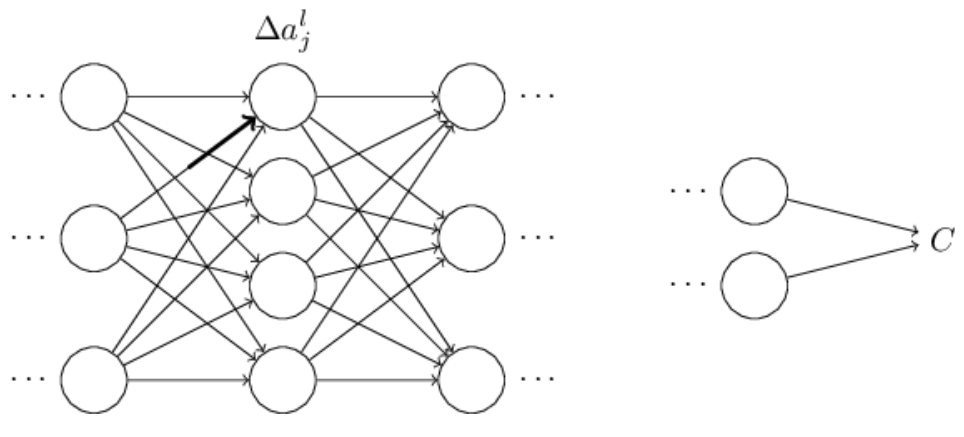
\includegraphics[width=0.8\linewidth]{img/NNprop1}
\caption{}
\label{NNprop1}
\end{subfigure}
\begin{subfigure}{0.9\textwidth}
\centering
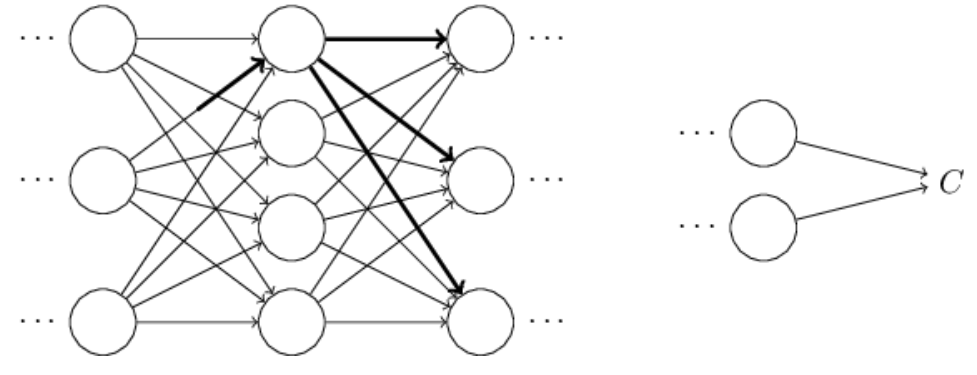
\includegraphics[width=0.8\linewidth]{img/NNprop2}
\caption{}
\label{NNprop2}
\end{subfigure}
\begin{subfigure}{0.9\textwidth}
\centering
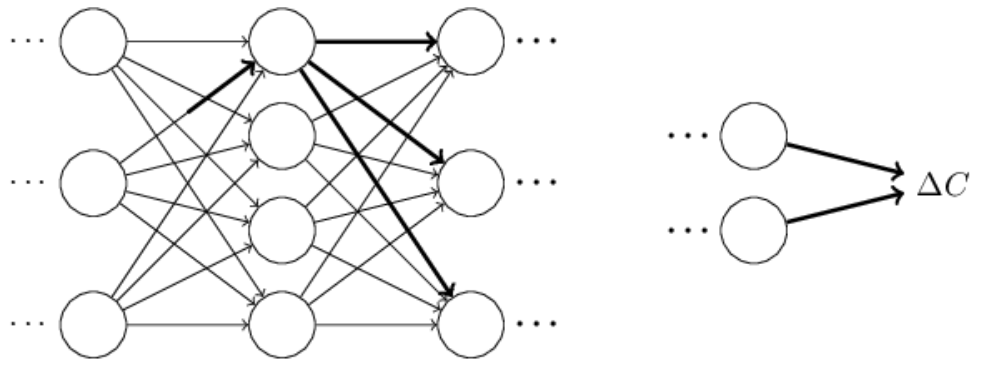
\includegraphics[width=0.8\linewidth]{img/NNprop3}
\caption{}
\label{NNprop3}
\end{subfigure}
\caption{Propagation when a single weight in the network has been changed.}
\label{weightCaange}
\end{figure}
The change $\Delta C$ in the cost function is related to the change in the weight (\autoref{weightCaange}):
\begin{equation}
\Delta C \approx \frac{\partial C}{\partial w_{jk}^\ell} \Delta w_{jk}^\ell
\label{DeltaC}
\end{equation}
This suggests that a possible approach to computing the partial derivative is to carefully track how a small change in the weight propagates to cause a small change in $C$. The change in the weight causes a small change in the neuron activation function (\autoref{NNprop1}). This change is given by
\begin{equation}
\Delta a_j^\ell \approx \frac{\partial a_j^\ell}{\partial w_{jk}^\ell}\Delta w_{jk}^\ell
\end{equation}

The change in activation will cause changes in all the activations in the next layer (\autoref{NNprop2}). We'll concentrate on the way just a single one of those activations is affected, say $a^{l+1}_q$. It will cause the following change:
\begin{equation}
\begin{aligned}
\Delta a^{l+1}_q \approx \frac{\partial a_q^{l+1}}{\partial a_j^\ell}\Delta a_j^\ell \Rightarrow\\
\Rightarrow \Delta a^{l+1}_q \approx \frac{\partial a_q^{l+1}}{\partial a_j^\ell} \frac{\partial a_j^{\ell}}{\partial w_{jk}^\ell}\Delta w_{jk}^\ell
\end{aligned}
\end{equation}
and this will propagate in the next layer as well. 
In fact, we can imagine a path all the way through the network from the updated weight to $C$, with each  change in activation causing a change in the next activation, and, finally, a change in the cost at the output. If the 
path goes through activations $a^\ell_j,a^{l+1}_q,\cdots,a^{L-1}_n,a^L_m$ then the resulting expression is:
\begin{equation}
\Delta C \approx \frac{\partial C}{\partial a^L_m} \frac{\partial a^L_m}{\partial a^{L-1}_n}\frac{\partial a^{L-1}_n}{\partial a^{L-2}_p}\cdots \frac{\partial a^{l+1}_q}{\partial a^\ell_j}\frac{\partial a^\ell_j}{\partial w^{\ell}_{jk}}\Delta w^{\ell}_{jk}
\end{equation}
This represents the change in $C$ due to changes in the activations along this particular path through the network. Of course, there are many paths by which a change in $w^\ell_{jk}$ can propagate to affect the cost, and we've been considering just a single path. To compute the total change in $C$ it is plausible that we should sum over all the possible paths between the weight and the final cost, i.e.,
\begin{equation}
\Delta C =\sum_{mnp\cdots q} \frac{\partial C}{\partial a^L_m}\frac{\partial a^L_m}{\partial a^{L-1}_n}\frac{\partial a^{L-1}_n}{\partial a^{L-2}_p}\cdots \frac{\partial a^{l+1}_q}{\partial a^\ell_j}\frac{\partial a^\ell_j}{\partial w^{\ell}_{jk}}\Delta w^{\ell}_{jk}
\end{equation}
Looking at \autoref{DeltaC}:
\begin{equation}
\frac{\partial C}{\partial w_{jk}^\ell} =  \sum_{mnp\cdots q} \frac{\partial C}{\partial a^L_m}\frac{\partial a^L_m}{\partial a^{L-1}_n}\frac{\partial a^{L-1}_n}{\partial a^{L-2}_p}\cdots \frac{\partial a^{l+1}_q}{\partial a^\ell_j}\frac{\partial a^\ell_j}{\partial w^{\ell}_{jk}}
\end{equation}
Now, the above equation looks complicated. However, it has a nice intuitive interpretation. We're computing the rate of change of $C$ with respect to a weight in the network. What the equation tells us is that every edge between two neurons in the network is associated with a rate factor which is just the partial derivative of one neuron's activation with respect to the other neuron's activation. The edge from the first weight to the first neuron has a rate factor $\frac{\partial a^\ell_j}{\partial w^\ell_{jk}}$. The rate factor for a path is just the product of the rate factors along the path. And the total rate of change $\frac{\partial C}{\partial w^\ell_{jk}}$ is just the sum of the rate factors of all paths from the initial weight to the final cost.

First, you could derive explicit expressions for all the individual partial derivatives. That's easy to do with a bit of calculus. Having done that, you could then try to figure out how to write all the sums over indices as matrix multiplications. This turns out to be tedious, and requires some persistence, but not extraordinary insight. After doing all this, and then simplifying as much as possible, what you discover is that you end up with exactly the backpropagation algorithm! And so you can think of the backpropagation algorithm as providing a way of computing the sum over the rate factor for all these paths. Or, to put it slightly differently, the backpropagation algorithm is a clever way of keeping track of small perturbations to the weights (and biases) as they propagate through the network, reach the output, and then affect the cost.

What about the other mystery - how backpropagation could have been discovered in the first place? In fact, if you follow the formal approach, you will discover a proof of backpropagation. Unfortunately, the proof is quite a bit longer and more complicated than the one I described earlier in this chapter. So how was that short (but more mysterious) proof discovered? What you find when you write out all the details of the long proof is that, after the fact, there are several obvious simplifications staring you in the face. You make those simplifications, get a shorter proof, and write that out. And then several more obvious simplifications jump out at you. So you repeat again. The result after a few iterations is the proof we saw earlier. There is one clever step required: the intermediate variables are activations like $a^{l+1}_q$. The clever idea is to switch to using weighted inputs, like $z^{l+1}_q$, as the intermediate variables. If you don't have this idea, and instead continue using the activations, the proof you obtain turns out to be slightly more complex than the proof given earlier in the chapter.

\subsection{Improving the way neural networks learn}
Some techniques can improve the learning procedure. There is a large variety of such techniques and they can act on the cost function, on the initialisation method or on the choice of hyper-parameters.

\subsubsection{The cross-entropy function}
We learn more quickly when we're decisively wrong, we learn more slowly when our errors are less well-defined. Yet, NNs have a lot of difficulty learning when they are badly wrong - far more difficulty than when it's just a little wrong. Why is learning so slow? And can we find a way of avoiding this slowdown? The NN changes the weights and bias at a rate determined by the partial derivatives: saying "learning is slow" is really the same as saying that those partial derivatives are small. To understand that, let's compute the partial derivatives. 

Consider a single neuron for a simple task: given the input $1$, output $0$. Recall that we're using the quadratic cost function $C= \frac{(y-a)^2}{2}$, where $a = \sigma(z)$:
\begin{equation}
\begin{aligned}
\frac{\partial C}{\partial w} &=(a-y)\sigma'(z) x = a\sigma'(z)\\
\frac{\partial C}{\partial b} &=(a-y)\sigma'(z) x = a\sigma'(z)\\
\end{aligned}
\end{equation}
where $y=0$ and $x=1$ by the definition of the problem. The sigmoid has the shape of \autoref{sigmDeriv}.
\begin{figure}
\centering
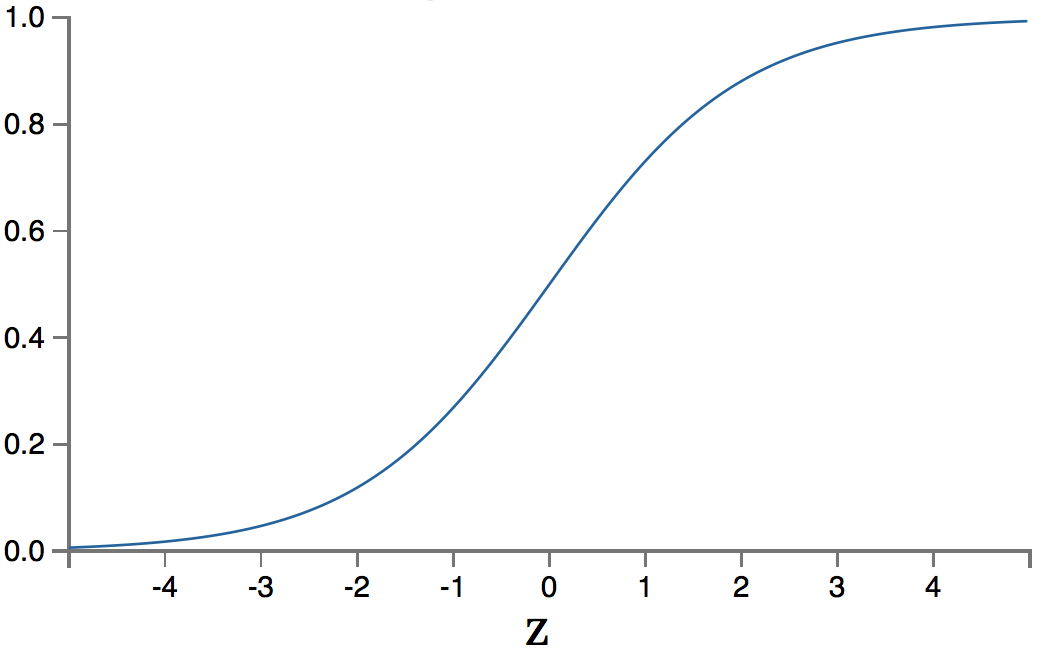
\includegraphics[scale=0.25]{img/sigmoid2}
\caption{Shape of the sigmoid function.}
\label{sigmDeriv}
\end{figure}
We can see from the graph that when the neuron's output is close to $1$, the curve gets very flat and the derivative gets very small, and so do the derivatives of the weight and bias. This is the origin of the learning slowdown. What's more, the learning slowdown occurs for essentially the same reason in more general neural networks, not just for the simple one considered.

The problem can be alleviated by replacing the quadratic cost function with the \tb{cross-entropy} function:
\begin{equation}
C =- \frac{1}{n} \sum_x \left[ y \ln a + (1-y) \ln(1-a)\right]
\end{equation}
where $n$ is the number of training data and $y$ the desired output. Two properties in particular make it reasonable to interpret the cross-entropy as a cost function. First, it's non-negative, that is, $C>0$,  since both logarithms are of numbers in the range $0$ to $1$. Second, if the neuron's actual output is close to the desired output for all training inputs $x$ (i.e., $y=0$ and $a\rightarrow 0$ or $y=1$ and $a\rightarrow 1$), then the cross-entropy will be close to zero.

The cross-entropy cost function has the benefit that, unlike the quadratic cost, it avoids the problem of learning slowing down. To see this, let's compute the partial derivative of the cross-entropy cost with respect to the weights:
\begin{equation}
\begin{aligned}
\frac{\partial C}{\partial w_j} &= - \frac{1}{n} \sum_x \br{ \frac{y}{\sigma(z)} -\frac{1-y}{1-\sigma(z)}} \frac{\partial\sigma}{\partial w_j} =  - \frac{1}{n} \sum_x \br{ \frac{y}{\sigma(z)} -\frac{1-y}{1-\sigma(z)}} \sigma'(z) x_j =\\
= \frac{\partial C}{\partial w_j} &= \frac{1}{n} \sum_x\frac{\cancel{\sigma'(z)} x_j}{\cancel{\sigma(z)\br{1-\sigma(z)}}}\br{\sigma(z) - y} = \frac{1}{n} \sum_x x_j \br{\sigma(z) - y}
\end{aligned} 
\end{equation}
This expression tells us that the rate at which the weight learns is controlled by $\sigma(z)-y$, i.e., by the error in the output. The larger the error, the faster the neuron will learn. This is just what we'd intuitively expect. In particular, it avoids the learning slowdown caused by the $\sigma'(z)$ term in the analogous equation for the quadratic cost. When we use the cross-entropy, the $\sigma'(z)$ term gets cancelled out, and we no longer need worry about it being small. Actually, as we'll see later, the cross-entropy was specially chosen to have just this property.

In a similar way, we can compute the partial derivative for the bias. One can easily verify that
\begin{equation}
\frac{\partial C}{\partial b} = \frac{1}{n} \sum_x \br{\sigma(z)-y}
\end{equation}

It's also easy to generalize the cross-entropy to many-neuron multi-layer networks. In particular, suppose $y=y_1,y_2,\cdots$ are the desired values at the output neurons, i.e., the neurons in the final layer, while $a^L_1,a^L_2,\cdots$ are the actual output values. Then we define the cross-entropy by
\begin{equation}
C = -\frac{1}{n}\sum_x \sum_j  \left[ y_j \ln a_j + (1-y_j) \ln(1-a_j)\right]
\end{equation}

It's common to define the cross-entropy for two probability distributions, $p_j$  and $p_q$, as $\sum_j p_j \ln q_j$. This definition may be connected the ones used in the NN, if we treat a single sigmoid neuron as outputting a probability distribution consisting of the neuron's activation a $a$ and its complement $1-a$. However, when we have many sigmoid neurons in the final layer, the vector of activations don't usually form a probability distribution and consequently the sum does not make any particular sense, since we're not working with probability distributions. Instead, you can think of it as a summed set of per-neuron cross-entropies, with the activation of each neuron being interpreted as part of a two-element probability distribution.

The cross-entropy is nearly always the better choice compared to the sigmoid, provided the output neurons are sigmoid neurons. To see why, consider that when we're setting up the network we usually initialize the weights and biases using some sort of randomization. It may happen that those initial choices result in the network being decisively wrong for some training input - that is, an output neuron will have saturated near $1$, when it should be $0$, or vice versa. If we're using the quadratic cost that will slow down learning. It won't stop learning completely, since the weights will continue learning from other training inputs, but it's obviously undesirable.

For the quadratic cost function, considering a single input:
\begin{equation}
\begin{aligned}
\frac{\pr C}{\pr w_{jk}^L} &= (a_{j}^L-y) \frac{\pr \sigma(z_{j}^L)}{\pr w_{jk}^L}  =(a_{j}^L-y)  \frac{\pr \sigma\br{\sum_k w_{jk}^L a_k{L-1}+b^L}}{\pr w_{jk}^L} =
\\&= (a_{j}^L-y) \sigma'(z_j^L) a_k^{L-1}
\end{aligned}
\end{equation}
where is $\sigma'(z_j^L)$ the term that slows down the learning.

For the cross-entropy function:
\begin{equation}
\begin{aligned}
\frac{\pr C}{\pr w_{jk}^L} &= \left[y \frac{1}{a_{j}^L} - \br{1-y}\frac{1}{1-a_{j}^L}\right]\frac{\pr a_j^L}{\pr w_{jk}^L} =\\
&=\left[\frac{y-a_{j}^L}{a_{j}^L\br{1-a_{j}^L}}\right]\frac{\pr a_j^L}{\pr w_{jk}^L} =\\
&=\left[\frac{y-a_{j}^L}{a_{j}^L\br{1-a_{j}^L}}\right] \sigma'(w_j^L)  \frac{\pr }{\pr w_{jk}^L} \br{\sum_k w_{jk}^L a_k^{L-1}+b_j^L}=\\
&=\left[\frac{y-a_{j}^L}{a_{j}^L\br{1-a_{j}^L}}\right] \sigma(w_j^L)\br{1-  \sigma(w_j^L)} a_k^{L-1}=\\
&=\left[\frac{y-a_{j}^L}{\cancel{a_{j}^L}\bcancel{{\br{1-a_{j}^L}}}}\right] \cancel{\sigma(w_j^L)}\bcancel{{\br{1-  \sigma(w_j^L)}}} a_k^{L-1}= \br{y-a_{j}^L} a_k^{L-1}
\end{aligned}
\end{equation}
The term $\sigma'(z_j^L)$ vanished and this avoids slowing down the learning. A simple variation on this analysis holds also for the biases.

$\sigma'(z_j^L)$ disappear also when using a quadratic cost function and having a linear activation function in the last layer:
\begin{equation}
\begin{aligned}
\frac{\pr C}{\pr w_{jk}^L} &= (a_{j}^L-y) \frac{\pr z_{j}^L}{\pr w_{jk}^L}  =(a_{j}^L-y) =
\\&= (a_{j}^L-y) a_k^{L-1}
\end{aligned}
\end{equation}

\paragraph{\tb{How does the learning rate change when switching from a quadratic cost function to a cross-entropy cost function?}} It's not possible to say precisely what it means to use the "same" learning rate when the cost function is changed. 

There is, incidentally, a very rough general heuristic for relating the learning rate for the cross-entropy and the quadratic cost. As we saw earlier, the gradient terms for the quadratic cost have an extra $\sigma'(x) = \sigma(x) \br{1-\sigma(x)}$ term in them. Suppose we average this over values for $\sigma(x)$:
\begin{equation}
\int_0^1 \sigma'(x) = \sigma(x) \br{1-\sigma(x)} d\sigma = \frac{1}{6}
\end{equation}
We see that (very roughly) the quadratic cost learns an average of $6$ times slower, for the same learning rate. This suggests that a reasonable starting point is to divide the learning rate for the quadratic cost by $6$. Of course, this argument is far from rigorous, and shouldn't be taken too seriously. Still, it can sometimes be a useful starting point.

\begin{proof}[\tb{Origin of the cross-entropy}]
To see how cross-entropy has been originally derived, suppose one has just found out that the term $\sigma'(z)$ is slowing down the learning process in equations \autoref{eq:NN1} and \autoref{eq:NN2}. We might wonder if it is possible to choose a cost function to make the term  $\sigma'(z)$ disappear. Basically one might want:

\begin{equation}
\begin{aligned}
\frac{\partial C}{\partial w} & =x \left( a^L - y\right)\\
\frac{\pr C}{\pr b} &=\left( a - y\right)
\end{aligned}
\end{equation}
From the chain-rule we have:
\begin{equation}
\frac{\pr C}{\pr b} =\frac{\pr C}{\pr a} \frac{\pr a}{\pr b }  =\frac{\pr C}{\pr a}\sigma'(z) = \frac{\pr C}{\pr a} \sz(1-\sz)
\end{equation}
Comparing the desired equation with the one of the chain rule, one gets
\begin{equation}
\frac{\pr C}{\pr a} = \frac{a-y}{a(1-a)} 
\end{equation}
Using the cover-up method (\autoref{coverupMethod}):
\begin{equation}
\frac{\pr C}{\pr a} = -\left[ y\ln a + (1-y)\ln(1-a)\right]+const
\end{equation}
To get the full cost function, we must average over all the training samples
\begin{equation}
\frac{\pr C}{\pr a} = -\frac{1}{n}\sum_x\left[y\ln a + (1-y)\ln(1-a)\right]+const
\end{equation}
where the constant here is the average of the individual constants for each training example.
\end{proof}

There is a standard way of interpreting the cross-entropy that comes from the field of information theory. Roughly speaking, the idea is that the cross-entropy is a measure of surprise. We get low surprise if the output $a$ is what we expect ($y$), and high surprise if the output is unexpected.

\subsubsection{Softmax neurons}
The idea of softmax is to define a new type of output layer for our neural networks. It begins in the same way as with a sigmoid layer, by forming the weighed inputs:
\newcommand{\jL}{_j^L}
\begin{equation}
z\jL = \sum_k w_{jk}^L a_k^L + b\jL
\end{equation}
However, we don't apply the sigmoid function to get the output. Instead, in a softmax layer we apply the so-called \tb{softmax function}.
\begin{equation}
a\jL = \frac{e^{z\jL}}{\sum_k e^{x_k^L}}
\end{equation}
In this way, the output activations are guaranteed to always sum up to $1$. The output activations are all positive, since the exponential function is positive. Combining these facts, we see that the output from the softmax layer is a set of positive numbers which sum up to $1$. In other words, the output from the softmax layer can be thought of as a probability distribution.

The softmax function and its properties have been described in \autoref{sssec:softmax}. There it has been shown how increasing the probability of one class automatically reduces the probabilities of the rest of the classes, keeping the overall sum $1$. Also note that for the softmax layer, the output of the $j$-th neuron is a function of the weights of the other neurons in the layer too:
\begin{equation*}
S(z\jL) = \frac{e^{\sum_k w_{jk}^L a_k^{L-1} +b_j^L}}{\sum_{\ell \in L}e^{\sum_k w_{\ell k}^L a_k^{L-1} +b_\ell^L}}
\end{equation*}

Now let us compute the derivatives for the $j$-th neuron:
\begin{equation}
\begin{aligned}
\frac{\pr C}{\pr b\jL} &= -\frac{1}{a\jL} \frac{e^{z\jL}\sum_{\ell \in L}e^{ w_{\ell}^L a^{L-1}+b_\ell^L} -e^{z\jL}e^{z\jL}}{\br{\sum_{\ell \in L}e^{ w_{\ell}^L a^{L-1} +b_\ell^L}}^2} \cancel{\frac{\pr z\jL}{\pr b\ell}} = \\
&= -\frac{1}{\cancel{a\jL}} \frac{ \cancel{e^{z\jL}} \br{\sum_{\ell \in L}e^{ w_{\ell}^L a^{L-1} +b\ell} -e^{z\jL}}}{\br{\sum_{\ell \in L}e^{ w_{\ell}^L a^{L-1} +b_\ell^L}}\cancel{^2}}= 1- a\jL
\end{aligned}
\end{equation}
and the weight:
\begin{equation}
\begin{aligned}
\frac{\pr C}{\pr w_{jk}^L} &= -\frac{1}{a\jL} \frac{e^{z\jL}\sum_{\ell \in L}e^{ w_{\ell}^L a^{L-1}+b_\ell^L} -e^{z\jL}e^{z\jL}}{\br{\sum_{\ell \in L}e^{ w_{\ell}^L a^{L-1} +b_\ell^L}}^2} \frac{\pr z\jL}{\pr w_{jk}^L} = \\
&= -\frac{1}{\cancel{a\jL}} \frac{ \cancel{e^{z\jL}} \br{\sum_{\ell \in L}e^{ w_{\ell}^L a^{L-1} +b\ell} -e^{z\jL}}}{\br{\sum_{\ell \in L}e^{ w_{\ell}^L a^{L-1} +b_\ell^L}}\cancel{^2}} a_k^{L-1}= \br{1- a\jL} a_k^{L-1}
\end{aligned}
\end{equation}

Therefore one might think to have a cost function at each output neuron that only looks at the considered class. This does not happen with the cross-entropy function where the terms $(1-\cdots)$ takes into account all the probability classes. Consider instead the \tb{$\log$-likelihood cost function} (\autoref{ssec:estimations}):
\begin{equation}
C = \sum_j y_j \log a^L_j -\ln a_y^L
\end{equation}

where $y$ is the desired output. The last equality holds because $y$ is one-hot-encoded vector, having a value equal to $1$ only for the $j$th element and $0$ for the others. Suppose we are training a MNIST classifier, and the input is an image of a $7$, then the log-likelihood cost is $-\ln a^L_7$.  The cost function will be close to $0$ when the output of  of the neuron is close to the desired value, i.e. $1$ for the $j$-th neuron and $0$ and very big when very far to this value (i.e. $0$).

Now consider the derivatives:
\begin{equation}
\begin{aligned}
\frac{\partial C}{\partial b_j^L} &= -\frac{1}{\cancel{a_j^L}}\frac{\cancel{e^{z_j}}\br{\sum_k e^{z_k}-e^{z)_j}}}{\br{\sum_k e^{z_k}}^{\cancel 2}} = a_j -1\\
\frac{\partial C}{\partial w_{j\ell}^L} &= -\frac{1}{\cancel{a_j^L}}\frac{a_\ell^{(L-1)}\cancel{e^{z_j}}\br{\sum_k e^{z_k}-e^{z)_j}}}{\br{\sum_k e^{z_k}}^{\cancel {2}}} = a_\ell^{(L-1)} \br{a_j^L -1}\\
\end{aligned}
\end{equation}
For the other neurons, one gets:
\begin{equation}
\begin{aligned}
\frac{\partial C}{\partial b_j^L} &= -\frac{1}{\cancel{a_i^L}}\frac{-\cancel{e^{z_i}} e^{z)_j}}{\br{\sum_k e^{z_k}}^{\cancel 2}} = a_j \\
\frac{\partial C}{\partial w_{j\ell}^L} &= -\frac{1}{\cancel{a_i^L}}\frac{-a_\ell^{(L-1)}\cancel{e^{z_i}}e^{z)_j}}{\br{\sum_k e^{z_k}}^{\cancel {2}}} = a_\ell^{(L-1)} a_j^L\\
\end{aligned}
\end{equation}

Although only a single output neuron contribute to the cost function, when backpropagating we need an expression also for the other neurons to update their parameters. The expressions can be generalised as:
\begin{equation}
\begin{aligned}
\frac{\partial C}{\partial b_j^L} &= a_j^L-y_j \\
\frac{\partial C}{\partial w_{j\ell}^L} &= -\frac{1}{\cancel{a_i^L}}\frac{-a_\ell^{(L-1)}\cancel{e^{z_i}}e^{z^L_j}}{\br{\sum_k e^{z^L_k}}^{\cancel {2}}} = a_\ell^{(L-1)} a_j^L-y_j\\
\end{aligned}
\end{equation}
where $y_j$ is the $j-th$ element of the $y$ desired output vector.

These equations are the same as the analogous expressions obtained in our earlier analysis of the cross-entropy, except the ones of cross-entropy are averaged on the number of the training example.  And, just as in the earlier analysis, these expressions ensure that we will not encounter a learning slowdown. In fact, it's useful to think of a softmax output layer with log-likelihood cost as being quite similar to a sigmoid output layer with cross-entropy cost. Given this similarity, should you use a sigmoid output layer and cross-entropy, or a softmax output layer and log-likelihood? In fact, in many situations both approaches work well. As a general point of principle, softmax plus log-likelihood is worth using whenever you want to interpret the output activations as probabilities. That's not always a concern, but can be useful with classification problems (like MNIST) involving disjoint classes.

Note that for the softmax layer:
\begin{equation}
\delta_j^L \equiv\frac{\partial C}{\partial z_j^L} = a_j^L-y_j 
\end{equation}

\subsubsection{Overfitting}
When overfitting the model will work well for the existing data, but will fail to generalize to new situations. The true test of a model is its ability to make predictions in situations it hasn't been exposed to before. Overfitting is a major problem in neural networks. This is especially true in modern networks, which often have very large numbers of weights and biases. To train effectively, we need a way of detecting when overfitting is going on, so we don't overtrain. And we'd like to have techniques for reducing the effects of overfitting. The obvious way to detect overfitting is to use the approach above, keeping track of accuracy on the test data as our network trains. If we see that the accuracy on the test data is no longer improving, then we should stop training. Of course, strictly speaking, this is not necessarily a sign of overfitting. It might be that accuracy on the test data and the training data both stop improving at the same time. Still, adopting this strategy will prevent overfitting. To avoid overfitting one way is to stop once classification accuracy has saturated. This strategy is called \tb{early stopping}.

Typically also the choice of hyperparameters might end up in overfitting, that is, we may end up finding hyper-parameters which fit particular peculiarities of the test-data, but where the performance of the network won't generalize to other data sets. To avoid this, data are divided in three groups: training, validation, and test. Training data are used to find the parameters of the model, validation is used to evaluate the choice of hyper-parameter and the test set are true evaluation of the model. Parameters should not be changed after looking at the test set.  This approach to finding good hyper-parameters is sometimes known as the \tb{hold out method}, since the validation data is kept apart or "held out" from the training data.

\tb{One should remember that whenever having the chance, the best method to reduce overfitting is increasing training data}. On the contrary, especially for simple tasks, one might thing to reduce the size of the network

\subsubsection{Regularization}
Increasing the samples and reducing the network size are not the only methods. Fortunately, there are other techniques which can reduce overfitting, even when having a fixed network and fixed training data. These are known as \tb{regularization techniques}.

Consider an $L2$ regularisation as already used for other algorithms.

\begin{equation}
\begin{aligned}
C &= -\frac{1}{n} \sum_{xj} \left[y_j \ln a_j^L +\br{1-y_j} \ln \br{1-a_j^L}\right] + \frac{\lambda}{2n} \sum_w w^2 = \\
&=C_0 +  \frac{\lambda}{2n} \sum_w w^2
\end{aligned}
\end{equation}
Again note that the regularisation term doesn't include the biases. Empirically, bias regularisation often doesn't change the results very much, so to some extent it's merely a convention whether to regularize the biases or not. However, it's worth noting that having a large bias doesn't make a neuron sensitive to its inputs in the same way as having large weights. And so we don't need to worry about large biases enabling our network to learn the noise in our training data. At the same time, allowing large biases gives our networks more flexibility in behaviour - in particular, large biases make it easier for neurons to saturate, which is sometimes desirable. For these reasons we don't usually include bias terms when regularizing.

Intuitively, the effect of regularization is to make the network prefer to learn small weights, all other things being equal. Large weights will only be allowed if they considerably improve the first part of the cost function. Put another way, regularization can be viewed as a way of compromising between finding small weights and minimizing the original cost function.

With such a cost function, the partial derivatives become:
\begin{equation}
\begin{aligned}
\frac{\pr C}{\pr w} &=\frac{\pr C_0}{\pr w}  + \frac{\lambda}{n} w \\
\frac{\pr C}{\pr b} &=\frac{\pr C_0}{\pr b}
\end{aligned}
\end{equation}
where they can be computed using backpropagation. The learning rules become:
\begin{equation}
\begin{aligned}
w\rightarrow &w -\eta \frac{\pr C_0}{\pr w} -\eta \frac{\lambda}{n} w = \br{1-\frac{\eta\lambda}{n}}w-\eta \frac{\pr C_0}{\pr w} \\
b\rightarrow &b- \eta \frac{\pr C_0}{\pr b}
\end{aligned}
\end{equation}
The rescaling $\br{1-\frac{\eta\lambda}{n}}$ is sometimes referred to as weight decay, since it makes the weights smaller. At first glance it looks as though this means the weights are being driven unstoppably toward zero. But that's not right, since the other term may lead the weights to increase, if so doing causes a decrease in the unregularized cost function.

The equations for the stochastic gradient become:
\begin{equation}
\begin{aligned}
w\rightarrow & \br{1-\frac{\eta\lambda}{n}}w-\frac{\eta}{m} \sum_x\frac{\pr C_x}{\pr w} \\
b\rightarrow &b-\frac{\eta}{m} \sum_x\frac{\pr C_x}{\pr b}
\end{aligned}
\end{equation}
Not only does the use of regularization suppress overfitting, it also improves the accuracy. It seems that, empirically, regularization causes networks to generalize better improving the classification accuracy and reducing the gap between training and test accuracy, apart from the effects of overfitting.

Empirically, when doing multiple runs of our MNIST networks, but with different (random) weight initializations, one will find that the unregularized runs will occasionally get "stuck", apparently caught in local minima of the cost function. The result is that different runs sometimes provide quite different results. By contrast, the regularized runs have provided much more easily replicable results. Heuristically, if the cost function is unregularized, then the length of the weight vector (its module) is likely to grow, all other things being equal. Over time this can lead to the weight vector module being very large indeed. This can cause the weight vector to get stuck pointing in more or less the same direction, since changes due to gradient descent only make tiny changes to the direction, when the length is long. This phenomenon might make it hard for the learning algorithm to properly explore the weight space, and consequently harder to find good minima of the cost function.

\paragraph{\tb{Why does regularisation help reduce overfitting?}} Smaller weights are said to have, in some sense, lower complexity, and so to provide a simpler and more powerful explanation for the data, and should thus be preferred. Let's see what this point of view means for neural networks. Suppose our network mostly has small weights, as will tend to happen in a regularized network. The smallness of the weights means that the behaviour of the network won't change too much if we change a few random inputs here and there. That makes it difficult for a regularized network to learn the effects of local noise in the data. Think of it as a way of making it so single pieces of evidence don't matter too much to the output of the network. Instead, a regularized network learns to respond to types of evidence which are seen often across the training set. By contrast, a network with large weights may change its behaviour quite a bit in response to small changes in the input. And so an unregularized network can use large weights to learn a complex model that carries a lot of information about the noise in the training data. In a nutshell, regularized networks are constrained to build relatively simple models based on patterns seen often in the training data, and are resistant to learning peculiarities of the noise in the training data. The hope is that this will force our networks to do real learning about the phenomenon at hand, and to generalize better from what they learn.

With that said, and keeping the need for caution in mind, it's an empirical fact that regularized neural networks usually generalize better than unregularized networks. No-one has yet developed an entirely convincing theoretical explanation for why regularization helps networks generalize. One can view regularization as something of a kludge. While it often helps, nobody has an entirely satisfactory systematic understanding of what's going on, merely incomplete heuristics and rules of thumb.

Considering the MNIST problem, a network generalize better than one might a priori expect. A network with 100 hidden neurons has nearly 80000 parameters, although having 50000 images in the training data. It's like trying to fit an 80000th degree polynomial to 50000 data points \footnote{\url{http://neuralnetworksanddeeplearning.com/chap3.html\#overfitting\_and\_regularization}}. By all rights, such a network should overfit terribly. And yet, such a network actually does a pretty good job generalizing. Why is that the case? It's not well understood. It has been conjectured \footnote{\url{http://yann.lecun.com/exdb/publis/pdf/lecun-01a.pdf}} that "the dynamics of gradient descent learning in multilayer nets has a `self-regularization' effect". This is exceptionally fortunate, but it's also somewhat disquieting that we don't understand why it's the case.

\subsubsection{Other techniques for regularization}
There are many regularization techniques other than $L2$ regularization. In this section three other approaches to reducing overfitting are briefly described: $L1$ regularization, dropout, and artificially increasing the training set size. 

\paragraph{\tb{$L1$ regularisation}}In this approach we modify the unregularized cost function by adding the sum of the absolute values of the weights.
\begin{equation}
C =C_0 + \frac{\lambda}{n}\sum_w \|w\|
\end{equation}
From this:
\begin{equation}
\begin{aligned}
\frac{\pr C}{\pr w} = \frac{\pr C_0}{\pr w} + \frac{\lambda}{n} sgn(w) 
\end{aligned}
\end{equation}
and so the update rule becomes:
\begin{equation}
w\rightarrow w-\eta \frac{\lambda}{n} sign(w) -\eta \frac{\pr C_0}{\pr w} 
\end{equation}
In both $L1$ and $L2$, the effect of regularization is to shrink the weights. But the way the weights shrink is different. In $L1$ regularization, the weights shrink by a constant amount toward $0$. In $L2$ regularization, the weights shrink by an amount which is proportional to $\|w\|$. And so when a particular weight has a large magnitude, $\|w\|$, $L1$ regularization shrinks the weight much less than $L2$ regularization does. By contrast, when $\|w\|$ is small, $L1$ regularization shrinks the weight much more than $L2$ regularization. The net result is that $L1$ regularization tends to concentrate the weight of the network in a relatively small number of high-importance connections, while the other weights are driven toward zero. Note that the partial derivative is not defined for $w=0$. What is typically done is just to apply the usual (unregularised) rule for stochastic gradient descent when $w=0$, i.e., to put $sign(0)=0$.

\paragraph{\tb{Dropout}} Unlike $L1$ and $L2$ regularization, dropout doesn't rely on modifying the cost function. Instead, in dropout we modify the network itself. Ordinarily, we'd train by forward-propagating the input through the network, and then backpropagating to determine the contribution to the gradient. With dropout, this process is modified. It starts by randomly (and temporarily) deleting half the hidden neurons in the network, while leaving the input and output neurons untouched. After doing this, we'll end up with a network along the following lines. We forward-propagate the input through the modified network, and then backpropagate the result, also through the modified network. After doing this over a mini-batch of examples, we update the appropriate weights and biases. We then repeat the process, first restoring the dropout neurons, then choosing a new random subset of hidden neurons to delete, estimating the gradient for a different mini-batch, and updating the weights and biases in the network. By repeating this process over and over, our network will learn a set of weights and biases. Of course, those weights and biases will have been learnt under conditions in which half the hidden neurons were dropped out. When we actually run the full network that means that twice as many hidden neurons will be active. To compensate for that, we halve the weights outgoing from the hidden neurons. In particular, imagine we train several different neural networks with no dropout, all using the same training data. Of course, the networks may not start out identical, and as a result after training they may sometimes give different results. When that happens we could use some kind of averaging or voting scheme to decide which output to accept. For instance, if we have trained five networks, and three of them are classifying a digit as a "3", then it probably really is a "3". The other two networks are probably just making a mistake. This kind of averaging scheme is often found to be a powerful (though expensive) way of reducing overfitting. The reason is that the different networks may overfit in different ways, and averaging may help eliminate that kind of overfitting. Heuristically, when we dropout different sets of neurons, it's rather like we're training different neural networks. And so the dropout procedure is like averaging the effects of a very large number of different networks. The different networks will overfit in different ways, and so, hopefully, the net effect of dropout will be to reduce overfitting.

A related heuristic explanation for dropout is given in one of the earliest papers to use the technique\footnote{\href{https://papers.nips.cc/paper/4824-imagenet-classification-with-deep-convolutional-neural-networks.pdf}{4824-imagenet-classification-with-deep-convolutional-neural-networks.pdf}}: "This technique reduces complex co-adaptations of neurons, since a neuron cannot rely on the presence of particular other neurons. It is, therefore, forced to learn more robust features that are useful in conjunction with many different random subsets of the other neurons." In other words, if we think of our network as a model which is making predictions, then we can think of dropout as a way of making sure that the model is robust to the loss of any individual piece of evidence. In this, it's somewhat similar to L1 and L2 regularization, which tend to reduce weights, and thus make the network more robust to losing any individual connection in the network. The technique was introduced by the paper \footnote{\url{https://arxiv.org/pdf/1207.0580.pdf}}.


\paragraph{\tb{Artificially expanding training data}} This idea is based on the fact that using vastly more training data - say, millions or even billions of handwriting samples, instead of just 50,000 - then one'd likely get considerably better performance, even from this very small network. Obtaining more training data is a great idea. Unfortunately, it can be expensive, and so is not always possible in practice. However, there's another idea which can work nearly as well, and that's to artificially expand the training data. Modifying pixel levels of the training set would get us new different images, although visually very similar. One can expand the training data by making many small rotations of all the MNIST training images, and then using the expanded training data to improve our network's performance. Some papers show positive results \footnote{\url{https://ieeexplore.ieee.org/document/1227801/}}. They expanded the training data, using not just rotations, as I described above, but also translating and skewing the images. By training on the expanded data set they increased their network's accuracy to 98.9 percent. They also experimented with what they called "elastic distortions", a special type of image distortion intended to emulate the random oscillations found in hand muscles. By using the elastic distortions to expand the data they achieved an even higher accuracy, 99.3 percent. Effectively, they were broadening the experience of their network by exposing it to the sort of variations that are found in real handwriting.

\subsubsection{Weight initialisation}
A way to initialise weights and biases is using Gaussian random variables, normalized to have mean $0$ and standard deviation $1$. Consider an neuron and suppose  half the input neurons are on, i.e., set to $1$, and half the input neurons are off, i.e., set to $0$. And so $z$ is a sum over a total of $501$ normalized Gaussian random variables, accounting for the $500$ weight terms and the extra bias term. Thus $z$ is itself distributed as a Gaussian with mean zero and standard deviation $\sqrt{501}$, that is \tb{a very broad Gaussian distribution, not sharply peaked at al}. The module of $z$ will likely be large: either $z>>1$ or $z<<-1$. If that's the case then the output $\sigma(z)$ from the hidden neuron will be very close to either $1$ or $0$. That means our hidden neuron will have saturated.  And when that happens, as we know, making small changes in the weights will make only absolutely miniscule changes in the activation of our hidden neuron. That miniscule change in the activation of the hidden neuron will, in turn, barely affect the rest of the neurons in the network at all, and we'll see a correspondingly miniscule change in the cost function. As a result, those weights will only learn very slowly when we use the gradient descent algorithm. While removing $\sigma'(z)$ helped to reduce the saturation in the output neurons, it did nothing for the saturation in the hidden neurons.
 
Suppose we have a neuron with $n_{in}$ input weights. Then we shall initialize those weights as Gaussian random variables with mean $0$ and standard deviation $1/\sqrt{n_{in}}$. That is, we'll squash the Gaussians down, making it less likely that our neuron will saturate. We'll continue to choose the bias as a Gaussian with mean $0$ and standard deviation $1$. Suppose, as we did earlier, that $500$ of the inputs are zero and $500$ are $1$. Then it's easy to show (see the exercise below) that $z$ has a Gaussian distribution with mean $0$ and standard deviation $\sqrt{3/2}=1.22$ (recall that the variance of a sum of independent random variables is the sum of the variances of the individual random variables and that the variance is the square of the standard deviation: $w~ N(0, \frac{1}{1000})$, so $\sigma_z^2 = 500/1000 + 1$ supposing only $500$ neurons active.

We'll continue to initialize the biases as before, as Gaussian random variables with a mean of $0$ and a standard deviation of $1$. This is okay, because it doesn't make it too much more likely that our neurons will saturate. In fact, it doesn't much matter how we initialize the biases, provided we avoid the problem with saturation. Some people go so far as to initialize all the biases to $0$, and rely on gradient descent to learn appropriate biases. But since it's unlikely to make much difference, we'll continue with the same initialization procedure as before.

With this technique, the final classification accuracy most of the times looks almost exactly the same, while the learning is much, much faster. However, in some examples where the long-run behaviour is significantly better with such an weight initialization. Thus it's not only the speed of learning which is improved, it's sometimes also the final performance.

\subsubsection{How to choose a neural network's hyper-parameters?}
In practice, when you're using neural nets to attack a problem, it can be difficult to find good hyper-parameters. There are some heuristics which can be used to set the hyper-parameters in a neural network.

\paragraph{\tb{Broad strategy}} When using neural networks to attack a new problem the first challenge is to get any non-trivial learning, i.e., for the network to achieve results better than chance. This can be surprisingly difficult, especially when confronting a new class of problem.  The way to go is to strip the problem down. Get rid of all the training and validation images except images which are 0s or 1s. Then try to train a network to distinguish 0s from 1s. Not only is that an inherently easier problem than distinguishing all ten digits, it also reduces the amount of training data by 80 percent, speeding up training by a factor of 5. That enables much more rapid experimentation, and so gives you more rapid insight into how to build a good network. You can further speed up experimentation by stripping your network down to the simplest network likely to do meaningful learning. If you believe a $[784, 10]$ network can likely do better-than-chance classification of MNIST digits, then begin your experimentation with such a network. It'll be much faster than training a $[784, 30, 10]$ network, and you can build back up to the latter.

You can get another speed up in experimentation by increasing the frequency of monitoring. Instead of using the full 10,000 image validation set to monitor performance, we can get a much faster estimate using just 100 validation images. It can be immensely frustrating to work with a network that's learning nothing. You can tweak hyper-parameters for days, and still get no meaningful response. And so it is advisable that during the early stages you should make sure you can get quick feedback from experiments. Intuitively, it may seem as though simplifying the problem and the architecture will merely slow you down. In fact, it speeds things up, since you much more quickly find a network with a meaningful signal. Once you've got such a signal, you can often get rapid improvements by tweaking the hyper-parameters. As with many things in life, getting started can be the hardest thing to do.

\paragraph{\tb{Learning rate}} Suppose we run three MNIST networks with three different learning rates, $0.025, 0.25$ and $2.5$, respectively and keep the other hyper-parameters the same. With $0.025$ the cost decreases smoothly until the final epoch. With $0.25$ the cost initially decreases, but after about $20$ epochs it is near saturation, and thereafter most of the changes are merely small and apparently random oscillations. Finally, with $2.5$ the cost makes large oscillations right from the start. To understand the reason for the oscillations, recall that stochastic gradient descent is supposed to step us gradually down into a valley of the cost function. However, if it is too large then the steps will be so large that they may actually overshoot the minimum, causing the algorithm to climb up out of the valley instead. The gradient descent in fact uses a first-order approximation to the cost function as a guide to how to decrease the cost. For large $\eta$, higher-order terms in the cost function become more important, and may dominate the behaviour, causing gradient descent to break down. This is especially likely as we approach minima and quasi-minima of the cost function, since near such points the gradient becomes small, making it easier for higher-order terms to dominate behaviour. When we choose $0.25$ the initial steps do take us toward a minimum of the cost function, and it's only once we get near that minimum that we start to suffer from the overshooting problem. And when we choose $0.025$ we don't suffer from this problem at all during the first $30$ epochs. Of course, choosing $\eta$ so small creates another problem, namely, that it slows down stochastic gradient descent. An even better approach would be to start with $0.25$, train for $20$ epochs, and then switch to $0.025$.
With this picture in mind, we can set $\eta$ as follows. First, we estimate the threshold value for $\eta$ at which the cost on the training data immediately begins decreasing, instead of oscillating or increasing. This estimate doesn't need to be too accurate. You can estimate the order of magnitude by starting with $\eta=0.01$. If the cost decreases during the first few epochs, then you should successively try $\eta=0.1,1.0,\cdots$ until you find a value for $\eta$ where the cost oscillates or increases during the first few epochs. Alternately, if the cost oscillates or increases during the first few epochs when $\eta=0.01$, then try $\eta=0.001,0.0001,\cdots$ until you find a value for $\eta$ where the cost decreases during the first few epochs. Following this procedure will give us an order of magnitude estimate for the threshold value of $\eta$. You may optionally refine your estimate, to pick out the largest value of $\eta$ at which the cost decreases during the first few epochs, say $\eta=0.5$ or $\eta=0.2$ (there's no need for this to be super-accurate). This gives us an estimate for the threshold value of $\eta$.
 
Some people use the training cost to pick $\eta$ appears in contradiction with what said earlier in this section, namely, that one should pick hyper-parameters by evaluating performance using our held-out validation data. In fact, use validation accuracy is used to pick the regularization hyper-parameter, the mini-batch size, and network parameters such as the number of layers and hidden neurons, and so on.  This choice is a personal preference, and is perhaps somewhat idiosyncratic. The reasoning is that the other hyper-parameters are intended to improve the final classification accuracy on the test set, and so it makes sense to select them on the basis of validation accuracy. However, the learning rate is only incidentally meant to impact the final classification accuracy. Its primary purpose is really to control the step size in gradient descent, and monitoring the training cost is the best way to detect if the step size is too big. With that said, this is a personal aesthetic preference. Early on during learning the training cost usually only decreases if the validation accuracy improves, and so in practice it's unlikely to make much difference which criterion you use.

\paragraph{\tb{Learning schedule}} It's often advantageous to vary the learning rate. Early on during the learning process it's likely that the weights are badly wrong. And so it's best to use a large learning rate that causes the weights to change quickly. Later, we can reduce the learning rate as we make more fine-tuned adjustments to our weights.  One natural approach is to use the same basic idea as early stopping. The idea is to hold the learning rate constant until the validation accuracy starts to get worse. Then decrease the learning rate by some amount, say a factor of two or ten. We repeat this many times, until, say, the learning rate is a factor of $1024$ (or $1000$) times lower than the initial value. Then we terminate.  For first experiments it is better to use a single, constant value for the learning rate. That'll get a good first approximation. Later, to obtain the best performance from a network, it's worth experimenting with a learning schedule\footnote{\url{https://arxiv.org/abs/1003.0358}}.

\paragraph{\tb{Use early stopping to determine the number of training epochs}} As we discussed earlier in the chapter, early stopping means that at the end of each epoch we should compute the classification accuracy on the validation data. When that stops improving, terminate. This makes setting the number of epochs very simple. In particular, it means that we don't need to worry about explicitly figuring out how the number of epochs depends on the other hyper-parameters. Instead, that's taken care of automatically. Furthermore, early stopping also automatically prevents us from overfitting. This is, of course, a good thing, although in the early stages of experimentation it can be helpful to turn off early stopping, so you can see any signs of overfitting, and use it to inform your approach to regularization. If we stop the first time the accuracy decreases then we'll almost certainly stop when there are more improvements to be had. A better rule is to terminate if the best classification accuracy doesn't improve for quite some time. This ensures that we don't stop too soon, in response to bad luck in training, but also that we're not waiting around forever for an improvement that never comes. Of course, this introduces a new hyper-parameter to optimize! In practice, however, it's usually easy to set this hyper-parameter to get pretty good results.

\paragraph{\tb{The regularization parameter $\lambda$}} A general suggestion is start initially with no regularization, and determining a value for $\eta$, as above. Using that choice of $\eta$, we can then use the validation data to select a good value for $\lambda$. Start by trialling $\lambda=1.0$, and then increase or decrease by factors of $10$, as needed to improve performance on the validation data. Once you've found a good order of magnitude, you can fine tune your value of $\lambda$. That done, you should return and re-optimize $\eta$  again.

\paragraph{\tb{Mini-batch size}} For on-line learning the mini-batch size would be $1$. This will cause significant errors in our estimate of the gradient. In fact, though, the errors turn out to not be such a problem. The reason is that the individual gradient estimates don't need to be super-accurate. All we need is an estimate accurate enough that our cost function tends to keep decreasing. It's possible to use matrix techniques to compute the gradient update for all examples in a mini-batch simultaneously, rather than looping over them. Depending on the details of your hardware and linear algebra library this can make it quite a bit faster to compute the gradient estimate for a mini-batch of (for example) size $100$, rather than computing the mini-batch gradient estimate by looping over the $100$ training examples separately. It might take (say) only $50$
 times as long, rather than $100$ times as long.  it's possible to use matrix techniques to compute the gradient update for all examples in a mini-batch simultaneously, rather than looping over them. Depending on the details of your hardware and linear algebra library this can make it quite a bit faster to compute the gradient estimate for a mini-batch of (for example) size $100$, rather than computing the mini-batch gradient estimate by looping over the $100$ training examples separately. It might take (say) only $50$ times as long, rather than $100$ times as long. choosing the best mini-batch size is a compromise. Too small, and you don't get to take full advantage of the benefits of good matrix libraries optimized for fast hardware. Too large and you're simply not updating your weights often enough. What you need is to choose a compromise value which maximizes the speed of learning. Fortunately, the choice of mini-batch size at which the speed is maximized is relatively independent of the other hyper-parameters (apart from the overall architecture), so you don't need to have optimized those hyper-parameters in order to find a good mini-batch size. The way to go is therefore to use some acceptable (but not necessarily optimal) values for the other hyper-parameters, and then trial a number of different mini-batch sizes, scaling $\eta$ as above. Plot the validation accuracy versus time (as in, real elapsed time, not epoch!), and choose whichever mini-batch size gives you the most rapid improvement in performance. With the mini-batch size chosen you can then proceed to optimize the other hyper-parameters.

\paragraph{\tb{Automated techniques}} Hand-optimization is a good way to build up a feel for how neural networks behave. However, and unsurprisingly, a great deal of work has been done on automating the process. A common technique is grid search, which systematically searches through a grid in hyper-parameter space. A review of both the achievements and the limitations of grid search (with suggestions for easily-implemented alternatives) may be found in a 2012 paper by Bergstra and Yoshua Bengio\footnote{\href{https://dl.acm.org/doi/10.5555/2503308.2188395}{Random search for hyper-parameter optimization, by James Bergstra and Yoshua Bengio (2012)}} . Many more sophisticated approaches have also been proposed: a particularly promising 2012 paper which used a Bayesian approach to automatically optimize hyper-parameters \footnote{\href{http://papers.nips.cc/paper/4522-practical-bayesian-optimization-of-machine-learning-algorithms.pdf}{Practical Bayesian optimization of machine learning algorithms, by Jasper Snoek, Hugo Larochelle, and Ryan Adams}}. The code from the paper is publicly available, and has been used with some success by other researchers.

In practice, there are relationships between the hyper-parameters. In practice, it helps to bounce backward and forward, gradually closing in good values. Above all, these heuristics are rules of thumb, not rules cast in stone. One should be on the lookout for signs that things aren't working, and be willing to experiment. 

There are a few particularly useful papers that synthesize and distill out much of this lore. Yoshua Bengio has a 2012 paper \footnote{\href{https://arxiv.org/abs/1206.5533}{Practical recommendations for gradient-based training of deep architectures, by Yoshua Bengio (2012)}} that gives some practical recommendations for using backpropagation and gradient descent to train neural networks, including deep neural nets. Another good paper is a 1998 paper \footnote{\href{http://yann.lecun.com/exdb/publis/pdf/lecun-98b.pdf}{Efficient BackProp, by Yann LeCun, Léon Bottou, Genevieve Orr and Klaus-Robert Müller (1998) by Yann LeCun, Léon Bottou, Genevieve Orr and Klaus-Robert Müller}}. Both these papers appear in an extremely useful 2012 book that collects many tricks commonly used in neural nets \footnote{\href{https://www.springer.com/gp/book/9783642352881}{Neural Networks: Tricks of the Trade, edited by Grégoire Montavon, Geneviève Orr, and Klaus-Robert Müller}}.

\subsubsection{Other techniques}
\paragraph{\tb{Variations on stochastic gradient descent}} One alternative is the \tb{Hessian technique}. By Taylor's theorem, the cost function can be approximated as:
\begin{equation}
C(w+\delta w) = C(w) +\sum_j \frac{\pr C}{\pr w_j}\Delta w_j +\frac{1}{2} \sum_{jk} \Delta w_j \frac{\pr^ 2}{\pr w_j \pr w_k} + \cdots = C(w) + \nabla C \Delta w +\frac{1}{2} \Delta w^T H  \Delta w +\cancel{\cdots}
\end{equation} 
Assuming that the Hessian matrix is positive definite, the minimum of the cost function over $\Delta w$ is given by the value:
\begin{equation}
\Delta w = - H^{-1} \nabla C
\end{equation}
obtained by taking the derivative. So moving from $w$ to $w+\Delta w$ should significantly decrease the cost function. That suggests a possible algorithm for minimizing the cost:
\begin{enumerate}
\item Choose a starting point, $w$.
\item Update $w$ to a new point $w'=w-H^{-1}\nabla C$.
\item Update $w'$ to a new point $w''=w'-H'^{-1} \nabla C'$
\item $\cdots$
\end{enumerate}
In practice it is still an approximation, so it's better to take smaller steps. We do this by repeatedly changing $w$  by an amount $\Delta w = -\eta H^{-1} \nabla C$.
There are theoretical and empirical results showing that Hessian methods converge on a minimum in fewer steps than standard gradient descent. In particular, by incorporating information about second-order changes in the cost function it's possible for the Hessian approach to avoid many pathologies that can occur in gradient descent. Furthermore, there are versions of the backpropagation algorithm which can be used to compute the Hessian. 
Unfortunately, while it has many desirable properties, it has one very undesirable property: it's very difficult to apply in practice. Part of the problem is the sheer size of the Hessian matrix. Suppose you have a neural network with $10^7$ weights and biases. Then the corresponding Hessian matrix will contain $10^7\times 10^7=10^{14}$ entries. However there are many variations on gradient descent which are inspired by Hessian optimization, but which avoid the problem with overly-large matrices. Let's take a look at one such technique, momentum-based gradient descent.

\paragraph{\tb{Momentum-based gradient descent}} The momentum technique modifies gradient descent in two ways that make it more similar to the physical picture of a ball rolling down into a valley. First, it introduces a notion of "velocity" for the parameters we're trying to optimize. The gradient acts to change the velocity, not (directly) the "position", in much the same way as physical forces change the velocity, and only indirectly affect position. Second, the momentum method introduces a kind of friction term, which tends to gradually reduce the velocity.

Let's give a more precise mathematical description. We introduce velocity variables $v_1, v_2, \cdots$, one for each $w_j$ (weights and biases). Then we replace the gradient descent update rule with:
\begin{equation}
\begin{aligned}
v \rightarrow v' &= \mu  v - \eta \nabla C \\
w \rightarrow w' &= w + v'
\end{aligned}
\end{equation}
In these equations, $\mu$ is a hyper-parameter which controls the amount of damping or friction in the system. To understand the meaning of the equations it's helpful to first consider the case where $\mu=1$, which corresponds to no friction. When that's the case, inspection of the equations shows that the "force" $\nabla C$ is now modifying the velocity, $v$, and the velocity is controlling the rate of change of $w$. Intuitively, we build up the velocity by repeatedly adding gradient terms to it. That means that if the gradient is in (roughly) the same direction through several rounds of learning, we can build up quite a bit of steam moving in that direction. Think, for example, of what happens if we're moving straight down a slope. With each step the velocity gets larger down the slope, so we move more and more quickly to the bottom of the valley. This can enable the momentum technique to work much faster than standard gradient descent. Of course, a problem is that once we reach the bottom of the valley we will overshoot. Or, if the gradient should change rapidly, then we could find ourselves moving in the wrong direction. That's the reason for the $\mu$ hyper-parameter. To be a little more precise, you should think of $1-\mu$ as the amount of friction in the system.

When $\mu=1$, as we've seen, there is no friction, and the velocity is completely driven by the gradient $\nabla C$. By contrast, when $\mu=0$ there's a lot of friction, the velocity can't build up, and one gets the usual equations. In practice, using a value of $\mu$ intermediate between $0$ and 1 can give us much of the benefit of being able to build up speed, but without causing overshooting. We can choose such a value for $\mu$ using the held-out validation data, in much the same way as we select $\eta$ and $\lambda$.

The the standard name for $\mu$ is badly chosen: it's called the \tb{momentum co-efficient}. This is potentially confusing, since $\mu$ is not at all the same as the notion of momentum from physics. Rather, it is much more closely related to friction. However, the term momentum co-efficient is widely used, so we will continue to use it.

A nice thing about the momentum technique is that it takes almost no work to modify an implementation of gradient descent to incorporate momentum. We can still use backpropagation to compute the gradients, just as before, and use ideas such as sampling stochastically chosen mini-batches. In this way, we can get some of the advantages of the Hessian technique, using information about how the gradient is changing. But it's done without the disadvantages, and with only minor modifications to our code. In practice, the momentum technique is commonly used, and often speeds up learning.

\paragraph{\tb{Other approaches to minimizing the cost function}}
The paper \ti{Efficient BackProp}\footnote{\href{http://yann.lecun.com/exdb/publis/pdf/lecun-98b.pdf}{Efficient BackProp, by Yann LeCun, Léon Bottou, Genevieve Orr and Klaus-Robert Müller (1998) by Yann LeCun, Léon Bottou, Genevieve Orr and Klaus-Robert Müller}} introduced earlier presents and compares several of these techniques, including conjugate gradient descent and the BFGS method (see also the closely related limited-memory BFGS method, known as L-BFGS). Another technique which has recently shown promising results \footnote{\href{http://www.cs.toronto.edu/~hinton/absps/momentum.pdf}{On the importance of initialization and momentum in deep learning, by Ilya Sutskever, James Martens, George Dahl, and Geoffrey Hinton (2012)}}. is Nesterov's accelerated gradient technique, which improves on the momentum technique. However, for many problems, plain stochastic gradient descent works well, especially if momentum is used, and so we'll stick to stochastic gradient descent through the remainder of this book.

\paragraph{\tb{Other models of artificial neurons}}
Networks built using other model neurons sometimes outperform sigmoid networks. Depending on the application, networks based on such alternate models may learn faster, generalize better to test data, or perhaps do both. Perhaps the simplest variation is the \tb{tanh} (pronounced "tanch") neuron, which replaces the sigmoid function by the hyperbolic tangent function. The output of a tanh neuron with input $x$, weight vector $w$, and bias $b$ is given by
\begin{equation}
\tanh (w \cdot x + b)
\end{equation}
where
\begin{equation}
\tanh(z) \equiv \frac{e^z - e^{-z}}{e^z + e^{-z}} \equiv \frac{\sinh(z)}{\cosh(z)}
\end{equation}

It turns out that this is very closely related to the sigmoid neuron: 
\begin{equation}
\begin{aligned}
\tanh(z) &= \frac{e^z - e^{-z}}{e^z + e^{-z}} = \frac{e^z }{e^z + e^{-z}} - \frac{ e^{-z}}{e^z + e^{-z}}= \frac{e^{2z} }{e^{2z} + 1} - \frac{ e^{-2z}}{1 + e^{-2z}} = \\ &=\sigma(2z) - \sigma(-2z) = 2\sigma(2z) - 1\\
\Rightarrow\sigma(z) &= \frac{1+\tanh{\frac{z}{2}}}{2}
\end{aligned}
\end{equation}
where the fact that $\sigma(z) + \sigma(-z) = 1$ has been used.
that is, $\tanh$ is just a rescaled version of the sigmoid function. We can also see graphically that the $tanh$ function has the same shape as the sigmoid function \autoref{tanh}.
 \begin{figure}
\centering
 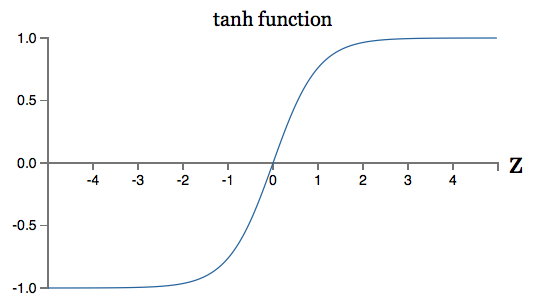
\includegraphics[scale=0.6]{img/tanh}
 \caption{$\tanh(z)$ activation function.}
 \label{tanh}
 \end{figure}
 \begin{figure}
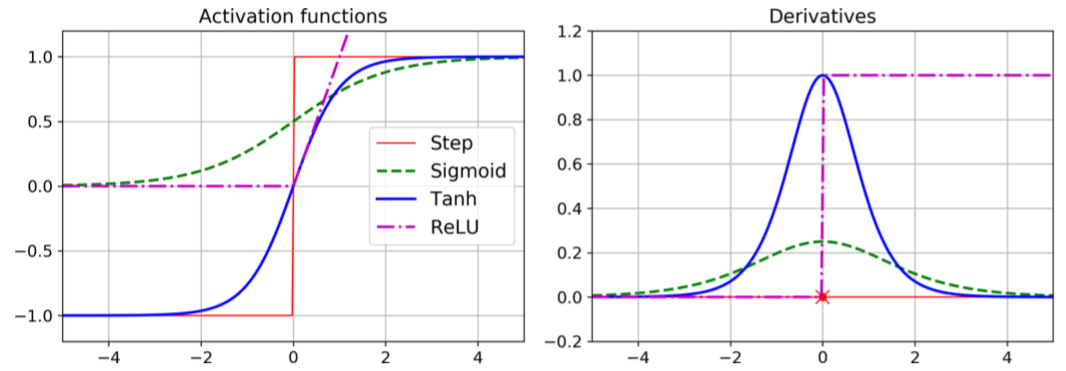
\includegraphics[scale=0.4]{img/activationFunctions}
\caption{Shape of different activation functions.}
\label{activationFunctions}
\end{figure}
 The output range of $\tanh$ is $[-1,1]$ instead of $[0,1]$. This means that if you're going to build a network based on tanh neurons you may need to normalize your outputs (and, depending on the details of the application, possibly your inputs) a little differently than in sigmoid networks. Furthermore, ideas such as backpropagation and stochastic gradient descent are as easily applied to a network of tanh neurons as to a network of sigmoid neurons.
 
 \paragraph{\tb{sigmoid versus hyperbolic tangent neurons}} There are theoretical arguments and some empirical evidence to suggest that the tanh sometimes performs better \footnote{\href{http://yann.lecun.com/exdb/publis/pdf/lecun-98b.pdf}{Efficient BackProp, by Yann LeCun, Léon Bottou, Genevieve Orr and Klaus-Robert Müller (1998) by Yann LeCun, Léon Bottou, Genevieve Orr and Klaus-Robert Müller}}, \footnote{\href{http://proceedings.mlr.press/v9/glorot10a/glorot10a.pdf}{Understanding the difficulty of training deep feedforward networks, by Xavier Glorot and Yoshua Bengio (2010)}}.
 
 Suppose we're using sigmoid neurons, so all activations in our network are positive and let's consider the weights input to one layer.The rules for backpropagation (see here) tell us that the associated gradient will $be a_k^l \delta^{\ell+1}_j$. Because the activations are positive the sign of this gradient will be the same as the sign of $\delta^{\ell+1}_j$. What this means is that if $\delta^{\ell+1}_j$ is positive then all the weights $w^{\ell+1}_{jk}$ will decrease during gradient descent, while if $\delta^{\ell+1}_j$ is negative then all the weights $w^{\ell+1}_{jk}$ will increase during gradient descent. In other words, all weights to the same neuron must either increase together or decrease together. That's a problem, since some of the weights may need to increase while others need to decrease. That can only happen if some of the input activations have different signs. That suggests replacing the sigmoid by an activation function, such as $\tanh$, which allows both positive and negative activations. Indeed, because $\tanh$ is symmetric about zero, $\tanh(-z)=-\tanh(z)$, we might even expect that, roughly speaking, the activations in hidden layers would be equally balanced between positive and negative. That would help ensure that there is no systematic bias for the weight updates to be one way or the other.

How seriously should we take this argument? While the argument is suggestive, it's a heuristic, not a rigorous proof that $\tanh$ neurons outperform sigmoid neurons. Perhaps there are other properties of the sigmoid neuron which compensate for this problem? Indeed, for many tasks the tanh is found empirically to provide only a small or no improvement in performance over sigmoid neurons. Unfortunately, we don't yet have hard-and-fast rules to know which neuron types will learn fastest, or give the best generalization performance, for any particular application.

\paragraph{\tb{Rectified linear neuron} or {Rectified linear unit}} The output of a rectified linear unit with input $x$, weight vector $w$, and bias $b$ is given by
\begin{equation}
max(0, w\cdot x+b)
\end{equation}
Graphically, it is shown in \autoref{relu}
\begin{figure}
\centering
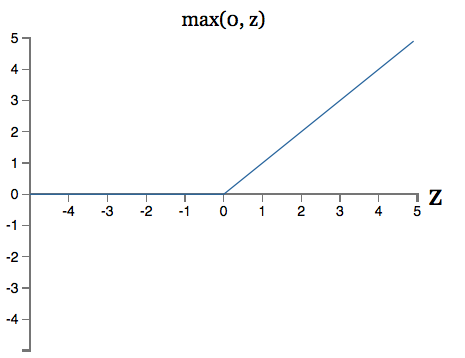
\includegraphics[scale=0.6]{img/relu}
\caption{Rectified linear activation function.}
\label{relu}
\end{figure}
When should you use rectified linear units instead of sigmoid or tanh neurons? Some recent work on image recognition \footnote{\href{http://neuralnetworksanddeeplearning.com/chap3.html\#other\_techniques}{What is the Best Multi-Stage Architecture for Object Recognition?, by Kevin Jarrett, Koray Kavukcuoglu, Marc'Aurelio Ranzato and Yann LeCun (2009)}}, \footnote{\href{http://proceedings.mlr.press/v15/glorot11a.html}{Deep Sparse Rectifier Neural Networks, by Xavier Glorot, Antoine Bordes, and Yoshua Bengio (2011)}}, \footnote{\href{https://papers.nips.cc/paper/4824-imagenet-classification-with-deep-convolutional-neural-networks.pdf}{ImageNet Classification with Deep Convolutional Neural Networks, by Alex Krizhevsky, Ilya Sutskever, and Geoffrey Hinton (2012)}}, \footnote{\href{https://www.cs.toronto.edu/~hinton/absps/reluICML.pdf}{Rectified Linear Units Improve Restricted Boltzmann Machines, by Vinod Nair and Geoffrey Hinton (2010)}}. However, as with tanh neurons, we do not yet have a really deep understanding of when, exactly, rectified linear units are preferable, nor why. To give you the flavor of some of the issues, recall that sigmoid neurons stop learning when they saturate, i.e., when their output is near either $0$ or $1$. As we've seen repeatedly in this chapter, the problem is that $\sigma'$ terms reduce the gradient, and that slows down learning. Tanh neurons suffer from a similar problem when they saturate. By contrast, increasing the weighted input to a rectified linear unit will never cause it to saturate, and so there is no corresponding learning slowdown. On the other hand, when the weighted input to a rectified linear unit is negative, the gradient vanishes, and so the neuron stops learning entirely. These are just two of the many issues that make it non-trivial to understand when and why rectified linear units perform better than sigmoid or tanh neurons.

\subsection{Universality of Neural Networks}
NNs are universal approximators of continous function. Continuous because NNs compute continuous functions of their input. However, even if the function we'd really like to compute is discontinuous, it's often the case that a continuous approximation is good enough. If that's so, then we can use a neural network. In practice, this is not usually an important limitation. A more precise statement of the universality theorem is that \tb{neural networks with a single hidden layer can be used to approximate any continuous function to any desired precision} \footnote{\href{http://www.dartmouth.edu/~gvc/Cybenko_MCSS.pdf}{Approximation by superpositions of a sigmoidal function, by George Cybenko (1989)}} , \footnote{\href{https://www.sciencedirect.com/science/article/abs/pii/0893608089900208}{Multilayer feedforward networks are universal approximators, by Kurt Hornik, Maxwell Stinchcombe, and Halbert White (1989)}}.

\subsection{Why are DNN hard to train? The vanishing gradient problem}
There are, mathematical proofs showing that for some functions very shallow circuits require exponentially more circuit elements to compute than do deep circuits. For instance, a famous series of papers in the early 1980s\footnote{\href{http://eccc.hpi-web.de/report/2012/137/}{On the correlation of parity and small-depth circuits}}. showed that computing the parity of a set of bits requires exponentially many gates, if done with a shallow circuit. On the other hand, if you use deeper circuits it's easy to compute the parity using a small circuit: you just compute the parity of pairs of bits, then use those results to compute the parity of pairs of pairs of bits, and so on, building up quickly to the overall parity. Deep circuits thus can be intrinsically much more powerful than shallow circuits. Also for NnN,just as in the case of circuits, there are theoretical results suggesting that deep networks are intrinsically more powerful than shallow networks (for certain problems and network architectures this is proved in \footnote{\href{https://arxiv.org/pdf/1312.6098.pdf}{On the number of response regions of deep feed forward networks with piece-wise linear activations, by Razvan Pascanu, Guido Montúfar, and Yoshua Bengio (2014)}}.

When trying to train a DNN with SGD and BP one will run into trouble. When we look closely, we'll discover that the different layers in our deep network are learning at vastly different speeds. In particular, when later layers in the network are learning well, early layers often get stuck during training, learning almost nothing at all. This stuckness isn't simply due to bad luck. Rather, we'll discover there are fundamental reasons the learning slowdown occurs, connected to our use of gradient-based learning techniques. As we delve into the problem more deeply, we'll learn that the opposite phenomenon can also occur: the early layers may be learning well, but later layers can become stuck. In fact, we'll find that there's an intrinsic instability associated to learning by gradient descent in deep, many-layer neural networks. This instability tends to result in either the early or the later layers getting stuck during training.

Let's assume that the extra hidden layers really could help in principle, and the problem is that our learning algorithm isn't finding the right weights and biases. We'd like to figure out what's going wrong in our learning algorithm, and how to do better. if one plots the rate of change of weights and bias in a multi-layer network, he will see that neurons in the last hidden layers will learn quite a bit faster than the neurons in the first hidden layers.
To determine whether this is a coincidence or not, it helps to have a global way of comparing the speed of learning in the first and second hidden layers. To do this, let's denote the gradient as $\delta^\ell_j=\frac{\pr C}{\pr b^\ell_j}$, i.e., the gradient for the $j$th neuron in the $\ell$-th layer. To have a rough idea one can check the lengths of the vector of each layer made up by the gradients of the neurons belonging to that layer. Doing shows that the neurons in the last hidden layers really are learning much faster than the neurons in the first hidden layers. The phenomenon is known as the vanishing gradient problem {\interfootnotelinepenalty10000{\footnote{\href{http://citeseerx.ist.psu.edu/viewdoc/summary?doi=10.1.1.24.7321}{Gradient flow in recurrent nets: the difficulty of learning long-term dependencies, by Sepp Hochreiter, Yoshua Bengio, Paolo Frasconi, and Jürgen Schmidhuber (2001)}}}. 

Sometimes the gradient gets much larger in earlier layers! This is the exploding gradient problem, and it's not much better news than the vanishing gradient problem. More generally, it turns out that the gradient in deep neural networks is unstable, tending to either explode or vanish in earlier layers. This instability is a fundamental problem for gradient-based learning in deep neural networks. It's something we need to understand, and, if possible, take steps to address.

\subsubsection{What's causing the vanishing gradient problem?}
To get insight into why the vanishing gradient problem occurs, let's consider the simplest deep neural network: one with just a single neuron in each layer as in \autoref{singleNeuronNetwork}.

\begin{figure}
\centering
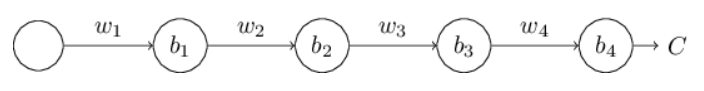
\includegraphics[scale=0.5]{img/singleNeuronNetwork}
\caption{Single neuron per layer network.}
\label{singleNeuronNetwork}
\end{figure}
We're going to study the gradient $\frac{\pr C}{\pr b_1}$ associated to the first hidden neuron. We'll figure out an expression for $\frac{\pr C}{\pr b_1}$, and $b_y$ studying that expression we'll understand why the vanishing gradient problem occurs.
\begin{equation}
\frac{\pr C}{\pr b_1} = \sigma'(z_1) \times w_2 \times \sigma'(z_2)\times w_3 \times \sigma'(z_3) \times w_4 \times \sigma'(z_4) \times \frac{\pr C}{\pr a_4}
\end{equation}
Imagine we make a small change $\Delta b_1$ in the bias $b_1$. That will set off a cascading series of changes in the rest of the network. First, it causes a change $\Delta a_1$ in the output from the first hidden neuron. That, in turn, will cause a change $\Delta z_2$ in the weighted input to the second hidden neuron. Then a change $\Delta a_2$ in the output from the second hidden neuron. And so on, all the way through to a change $\Delta C$ in the cost at the output. We have

\begin{equation}
\frac{\pr C}{\pr b_1} = \frac{\Delta C}{\Delta b_1}
\end{equation}

Let's think about how $\Delta b_1$ causes the output $a_1 $from the first hidden neuron to change. We have $a_1=\sigma(z_1)=\sigma(w1a0+b_1)$, so 
\begin{equation}
\Delta a_1\approx \frac{\pr \sigma(w_1a_0+b_1)}{\pr b_1}\Delta b_1 = \sigma'(z_1)\Delta b_1. 
\end{equation}
That $\sigma'(z_1)$ term should look familiar: it's the first term in our claimed expression for the gradient $\frac{\pr C}{\pr b_1}$. Intuitively, this term converts a change $\Delta b_1$ in the bias into a change $\Delta a_1$ in the output activation. That change $\Delta a_1$ in turn causes a change in the weighted input $z_2=w_2a_1+b_2$ to the second hidden neuron:
\begin{equation}
\Delta z_2\approx=\frac{\pr z_2}{\pr a_1} \Delta a_1 = w_2\Delta a_1.
\end{equation}
Combining our expressions for $\Delta z_2$ and $\Delta a_1$, we see how the change in the bias $b_1$ propagates along the network to affect $z_2$:
\begin{equation}
\Delta z_2\approx\sigma'(z_1)w_2\Delta b_1.
\end{equation}
Again, that should look familiar: we've now got the first two terms in our claimed expression for the gradient $\frac{\pr C}{\pr b_1}$.

We can keep going in this fashion, tracking the way changes propagate through the rest of the network. At each neuron we pick up a $\sigma'(z_j)$ term, and through each weight we pick up a $w_j$ term. The end result is an expression relating the final change $\Delta C$
 in cost to the initial change $\Delta b_1$ in the bias:
\begin{equation}
\Delta C\approx\sigma'(z_1)w_2\sigma'(z_2)\cdots\sigma'(z_4)\frac{\pr C}{\pr a_4}\Delta b_1
\end{equation}. 
Dividing by $\Delta b_1$ we do indeed get the desired expression for the gradient:
\begin{equation}
\frac{\pr C}{\pr b_1}=\sigma'(z_1)w_2\sigma'(z_2)\cdots\sigma'(z_4)\frac{\pr C}{\pr a_4}
\end{equation}

Why the vanishing gradient problem occurs: To understand why the vanishing gradient problem occurs, let's explicitly write out the entire expression for the gradient:
\begin{equation}
\frac{\pr C}{\pr b_1}=\sigma'(z_1)w_2\sigma'(z_2)w3\sigma'(z3)w_4\sigma'(z_4)\frac{\pr C}{\pr a_4}
\end{equation} 
Excepting the very last term, this expression is a product of terms of the form $w_j\sigma'(z_j)$. The derivative reaches a maximum at $\sigma'(0)=1/4$.  Now, if we use our standard approach to initializing the weights in the network, then we'll choose the weights using a Gaussian with mean $0$ and standard deviation $1$. So the weights will usually satisfy $\|w_j\|<1$. Putting these observations together, we see that $\|w_j \sigma'(z_j)\|<1/4$. And when we take a product of many such terms, the product will tend to exponentially decrease: the more terms, the smaller the product will be. This is starting to smell like a possible explanation for the vanishing gradient problem.
\begin{figure}
\centering
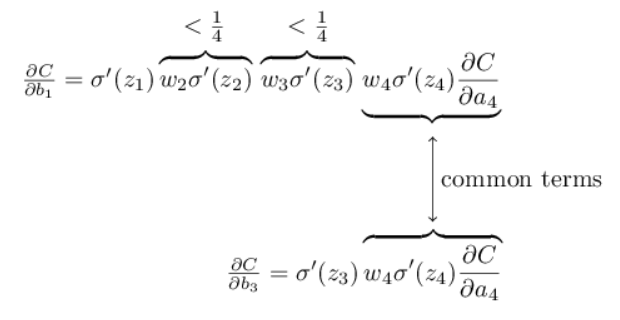
\includegraphics[scale=0.5]{img/vanishinggradient}
\caption{Comparison between the gradients of first and 4-th layer.}
\label{vanishing}
\end{figure}
From \autoref{vanishing}, the gradient in the first layer will be approximately $1/16$ smaller than the one in the fourth layer.

Of course, this is an informal argument, not a rigorous proof that the vanishing gradient problem will occur. There are several possible escape clauses. In particular, we might wonder whether the weights $w_j$ could grow during training. If they do, it's possible the terms $w_j\sigma'(z_j)$ in the product will no longer have a module smaller than $1$. Indeed, if the terms get large enough - greater than $1$ - then we will no longer have a vanishing gradient problem. Instead, the gradient will actually grow exponentially as we move backward through the layers. Instead of a vanishing gradient problem, we'll have an exploding gradient problem.

\paragraph{\tb{The exploding gradient problem}} There are two steps to getting an exploding gradient. First, we choose all the weights in the network to be large (for example $100$).Second, we'll choose the biases so that the $\sigma'(z_j)$ terms are not too small. That's actually pretty easy to do: all we need do is choose the biases to ensure that the weighted input to each neuron is $z_j=0$ (and so $\sigma'(z_j)=1/4$). So, for instance, we want $z_1=w_1a_0+b_1=0$. We can achieve this by setting $b_1=-100\cdot a_0$. We can use the same idea to select the other biases. When we do this, we see that all the terms $w_j\sigma'(z_j)$ are equal to $100\cdot 1/4=25$. With these choices we get an exploding gradient.

\paragraph{\tb{The unstable gradient problem}} The fundamental problem here isn't so much the vanishing gradient problem or the exploding gradient problem. It's that the gradient in early layers is the product of terms from all the later layers. When there are many layers, that's an intrinsically unstable situation. The only way all layers can learn at close to the same speed is if all those products of terms come close to balancing out. Without some mechanism or underlying reason for that balancing to occur, it's highly unlikely to happen simply by chance. In short, the real problem here is that neural networks suffer from an unstable gradient problem. As a result, if we use standard gradient-based learning techniques, different layers in the network will tend to learn at wildly different speeds. To avoid the vanishing gradient problem we need $|w\sigma'(z)|\ge 1$. You might think this could happen easily if $w$ is very large. However, it's more difficult than it looks. The reason is that the $\sigma'(z)$ term also depends on $w$: $\sigma'(z)=\sigma'(wa+b)$. So when we make $w$ large, we need to be careful that we're not simultaneously making $\sigma'(wa+b)$ small. That turns out to be a considerable constraint. The reason is that when we make $w$ large we tend to make $wa+b$ very large. Looking at the graph of $\sigma'$ you can see that this puts us off in the "wings" of the $\sigma'$function, where it takes very small values. The only way to avoid this is if the input activation falls within a fairly narrow range of values (this qualitative explanation is made quantitative in the first problem below). Sometimes that will chance to happen. More often, though, it does not happen. And so in the generic case we have vanishing gradients.

Much the same behaviour presented above occurs also in more complex networks. 

\paragraph{\tb{The prevalence of the vanishing gradient problem}} We've seen that the gradient can either vanish or explode in the early layers of a deep network. In fact, when using sigmoid neurons the gradient will usually vanish. 

A paper studied \footnote{\href{http://www.cs.toronto.edu/~hinton/absps/momentum.pdf}{On the importance of initialization and momentum in deep learning by Ilya Sutskever, James Martens, George Dahl and Geoffrey Hinton (2013)}} the impact on deep learning of both the random weight initialization and the momentum schedule in momentum-based stochastic gradient descent. In both cases, making good choices made a substantial difference in the ability to train deep networks.

